\vspace{-0.1in}
\section{Kernel Observers}\label{sec:observers}

This section outlines our modeling framework and presents theoretical results associated with the number of sampling locations required for monitoring functional evolution. 
\vspace{-0.1in}
\subsection{Problem Formulation}\label{sec:formulation}
We focus on predictive inference of a time-varying stochastic process, whose mean $f$ evolves temporally as $f_{\tindex+1} \sim \mathbb{F}(f_{\tindex},\eta_{\tindex})$, where $\mathbb{F}$ is a distribution varying with time $\tindex$ and exogenous inputs $\eta$. Our approach builds on the fact that in several cases, temporal evolution can be hierarchically separated from spatial functional evolution. A classical and quite general example of this is the \emph{abstract evolution equation} (AEO), which can be defined as the evolution of a function $\banachfunc$ embedded in a Banach space $\banachspace$: $\dot{\banachfunc}(t) = \banachop\banachfunc(t)$, subject to $\banachfunc(0)= \banachfunc_0$, and $\banachop:\banachspace\to\banachspace$ determines spatiotemporal transitions of $\banachfunc\in\banachspace$ \cite{brezis2010functional}. This model of spatiotemporal evolution is very general (AEOs, for example, model many PDEs), but working in Banach spaces can be computationally taxing.  A simple way to make the approach computationally realizable is to place restrictions on $\banachspace$: in particular, we restrict the sequence $f_{\tindex}$ to lie in a reproducing kernel Hilbert space (RKHS), the theory of which provides powerful tools for generating flexible classes of functions with relative ease \cite{RasmussenWilliams2005}.
In a kernel-based model, $\kernel:\dom\times\dom\to\R$ is a positive-definite Mercer kernel on a domain $\dom$ that models the covariance between any two points in the input space,  
and implies the existence of a smooth map $\fmap:\dom\to\fspace$, where $\fspace$ is an RKHS with the property $\kernel(x,y) = \Kiprod{x}{y}$. The key insight behind the proposed model is that spatiotemporal evolution in the input domain corresponds to temporal evolution of the mixing weights of a kernel model alone in the functional domain. Therefore, $f_{\tindex}$ can be modeled by tracing the evolution of its mean embedded in a RKHS using switched ordinary differential equations (ODE) when the evolution is continuous, or switched difference equations when it is discrete (Figure \ref{fig:hilbert_evolution}). 
The advantage of this approach is that it allows us to utilize powerful ideas from systems theory for deriving necessary and sufficient conditions for spatiotemporal monitoring. 
\begin{figure}
\centering
\begin{minipage}{0.45\textwidth}
\centering
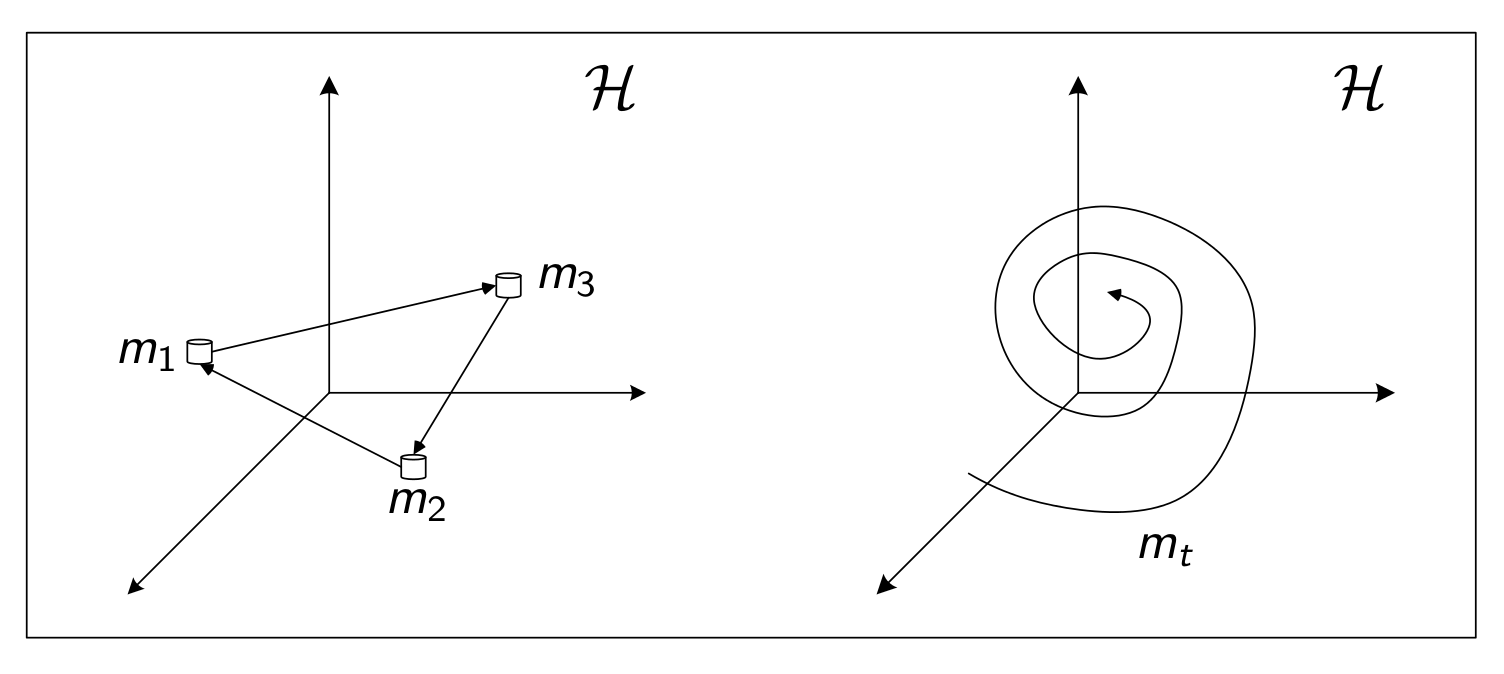
\includegraphics[height=1.0in]{figures/model.png}
\caption{\small{Two types of Hilbert space evolutions. Left: discrete switches in RKHS $\fspace$; Right: smooth evolution in $\fspace$.}}
\label{fig:hilbert_evolution}           
\end{minipage}\hfill
\begin{minipage}{0.45\textwidth}
\centering
\subfloat[\small{1-shaded (Def. \ref{def:shaded})}]{
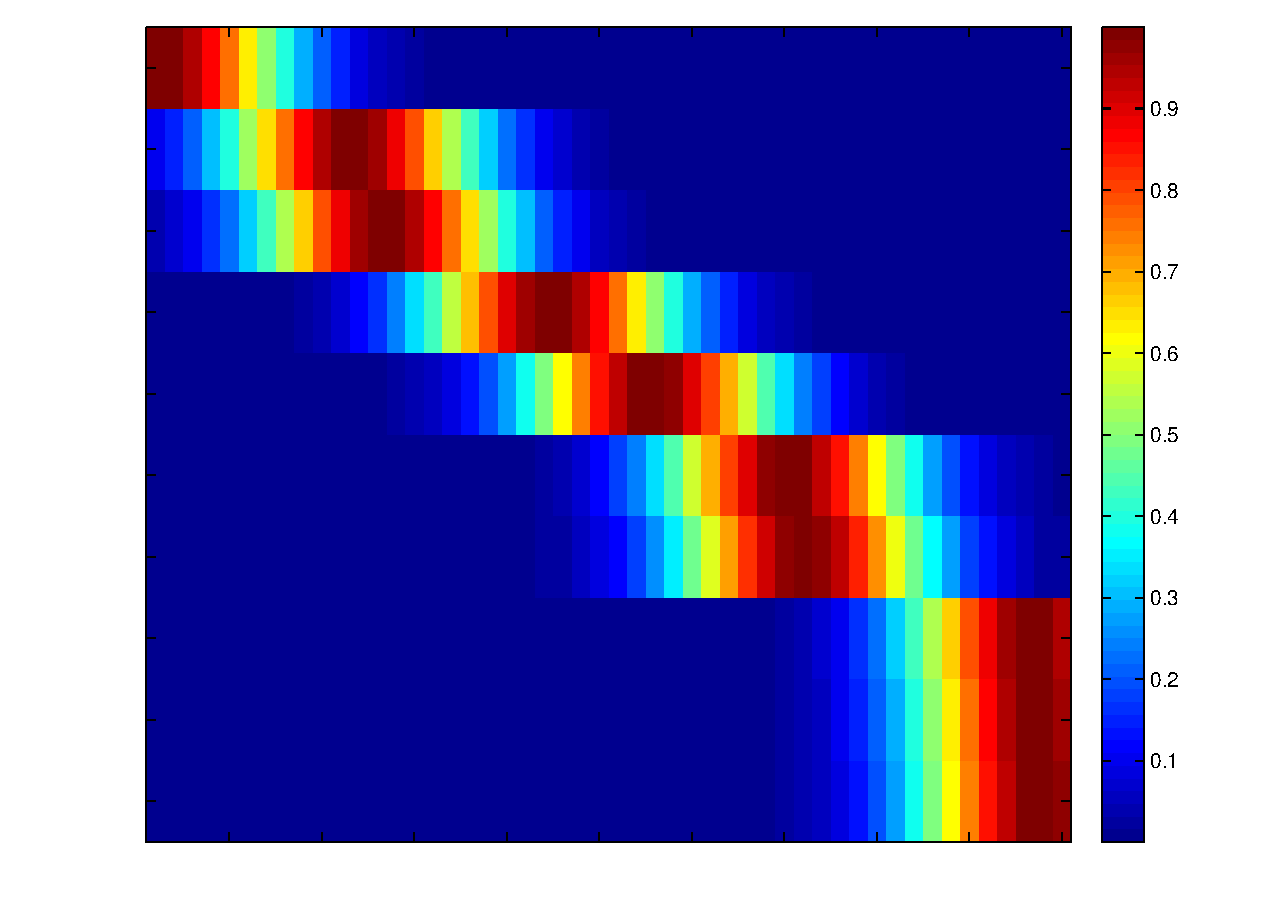
\includegraphics[width=0.47\columnwidth]{shaded_kmat.pdf} \label{fig:shadeda}}
\subfloat[\small{2-shaded (Eq. \eqref{empKShadFull})}]{
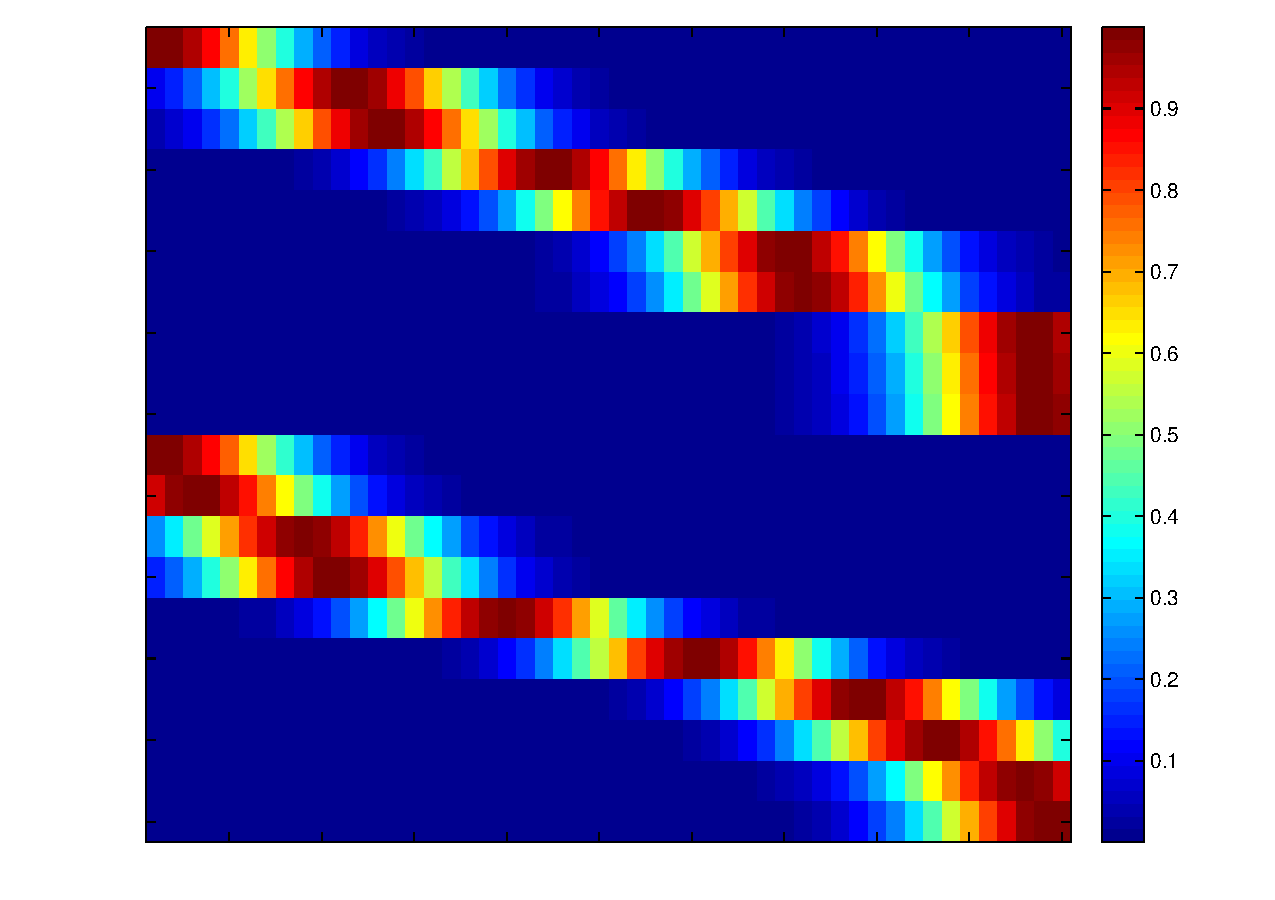
\includegraphics[width=0.47\columnwidth]{shaded_kmat_multiple.pdf} \label{fig:shadedb}}
\caption{\small{Shaded observation matrices for dictionary of atoms. Each row represents a sensing location with the color map indicating the evaluation of kernel function w.r.t the others points in the domain.}}
\label{fig:shaded}
\end{minipage}
\end{figure}
% \begin{figure}
%  \centering
%  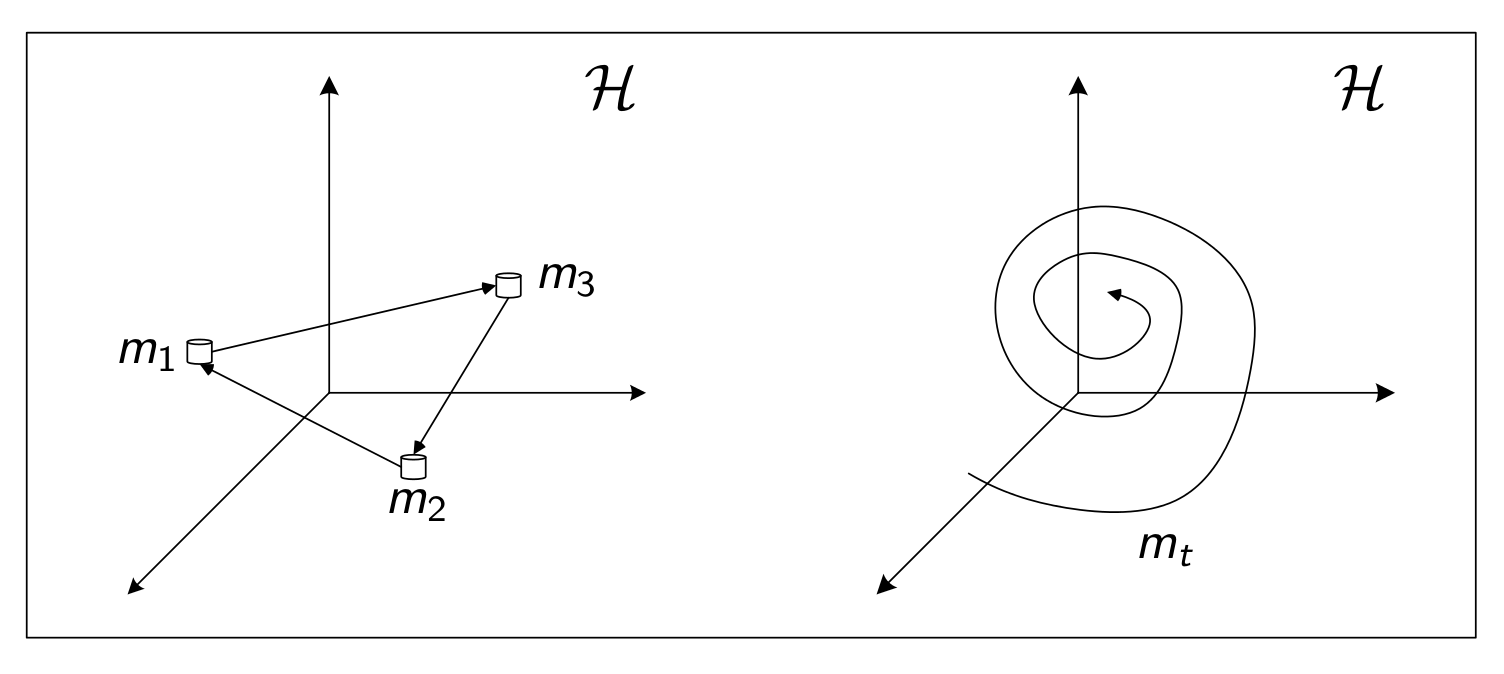
\includegraphics[height=2.0in]{figures/model.png}
% \caption{\small{Two types of Hilbert space evolutions. Left: discrete switches in RKHS $\fspace$; Right: smooth evolution in $\fspace$.}}
% \label{fig:hilbert_evolution}
% \end{figure} 
% \begin{figure}
%  \centering
%  \subfloat[\small{1-shaded (Definition \ref{def:shaded})}]{
% 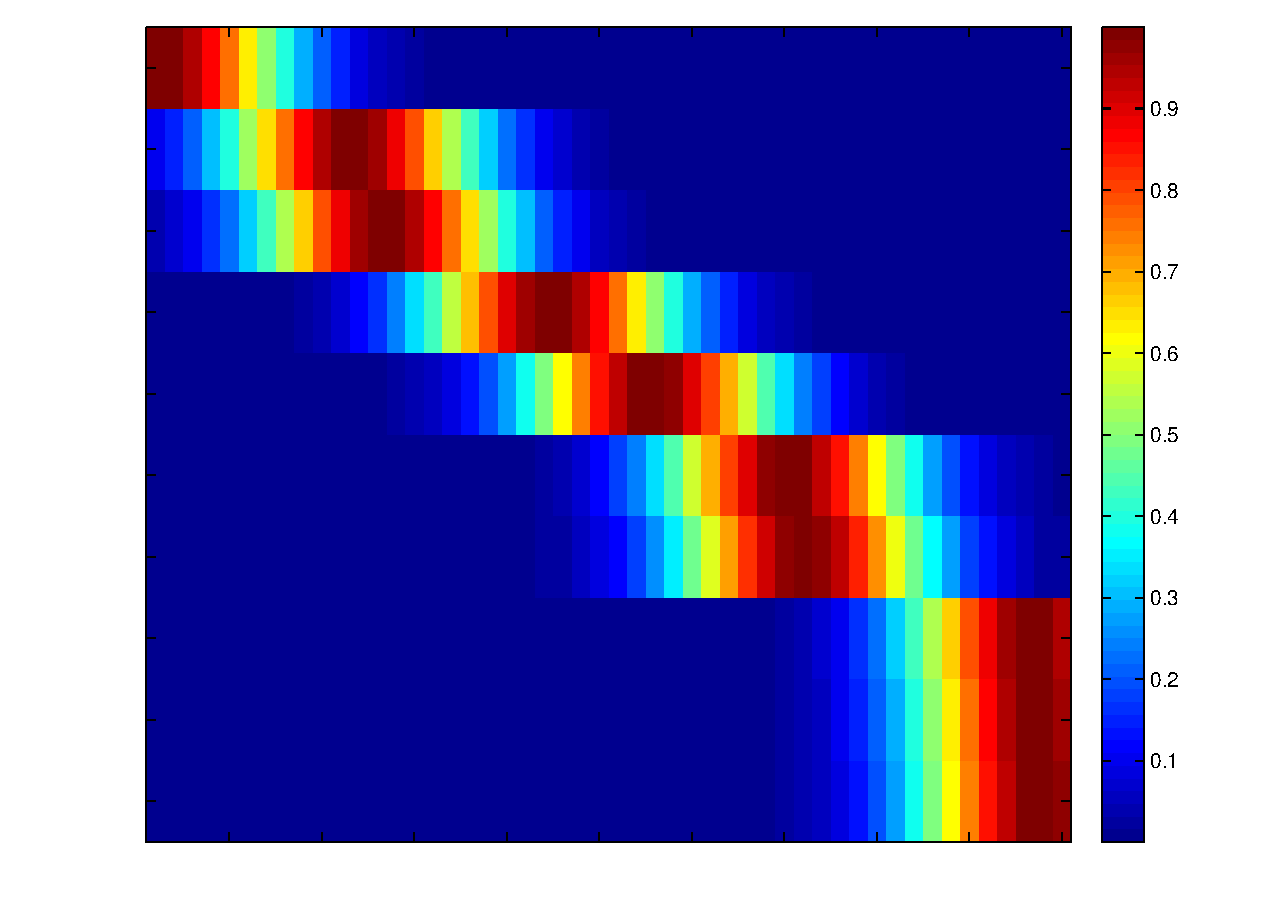
\includegraphics[width=0.4\columnwidth]{shaded_kmat.pdf} \label{fig:shadeda}}
% \subfloat[\small{2-shaded (Eq. \eqref{empKShadFull})}]{
% 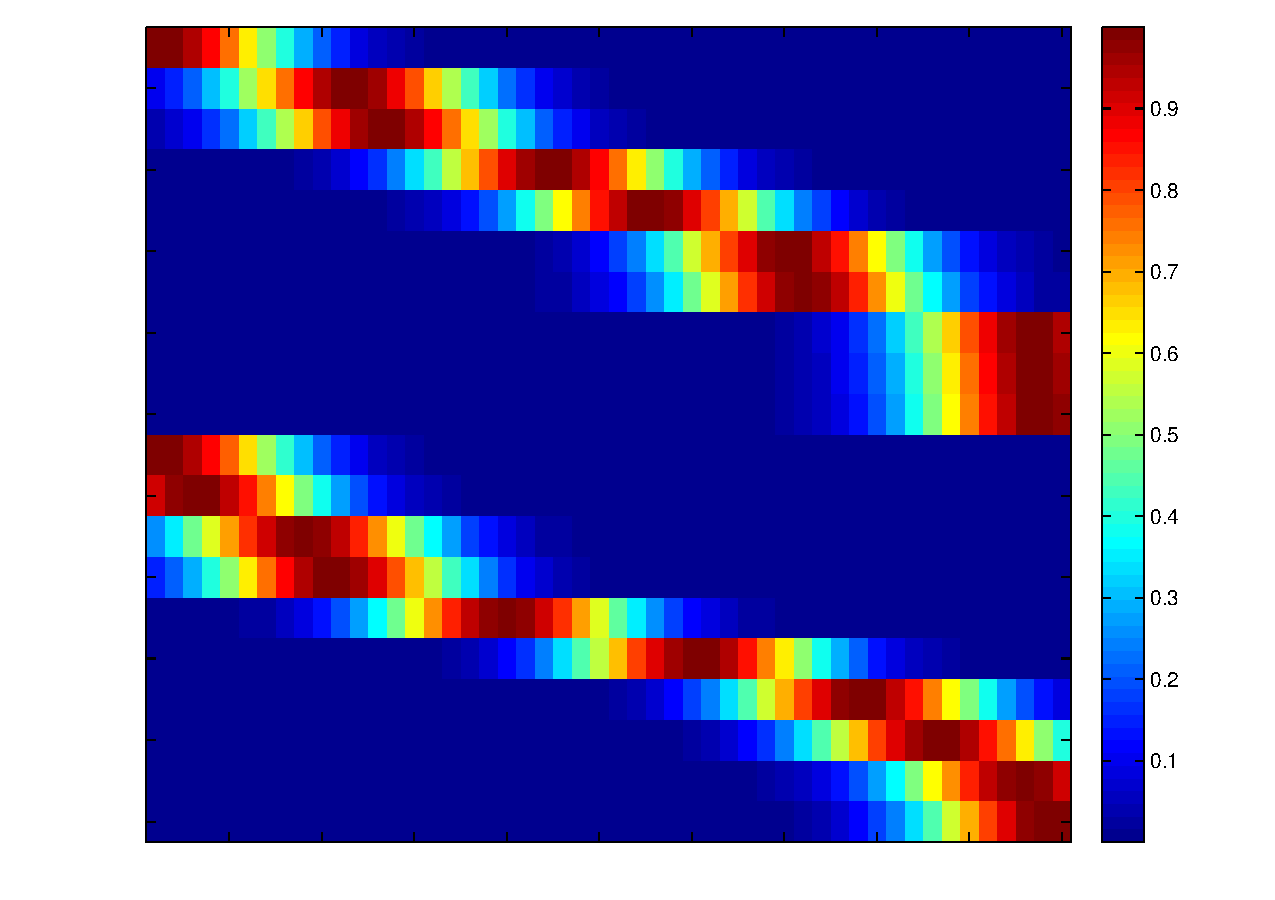
\includegraphics[width=0.4\columnwidth]{shaded_kmat_multiple.pdf} \label{fig:shadedb}}
% \caption{\small{Shaded observation matrices for dictionary of atoms.}}
% \label{fig:shaded}
% \end{figure}

\begin{figure}[t]
\centering
\subfloat[\small{Gaussian}]{
 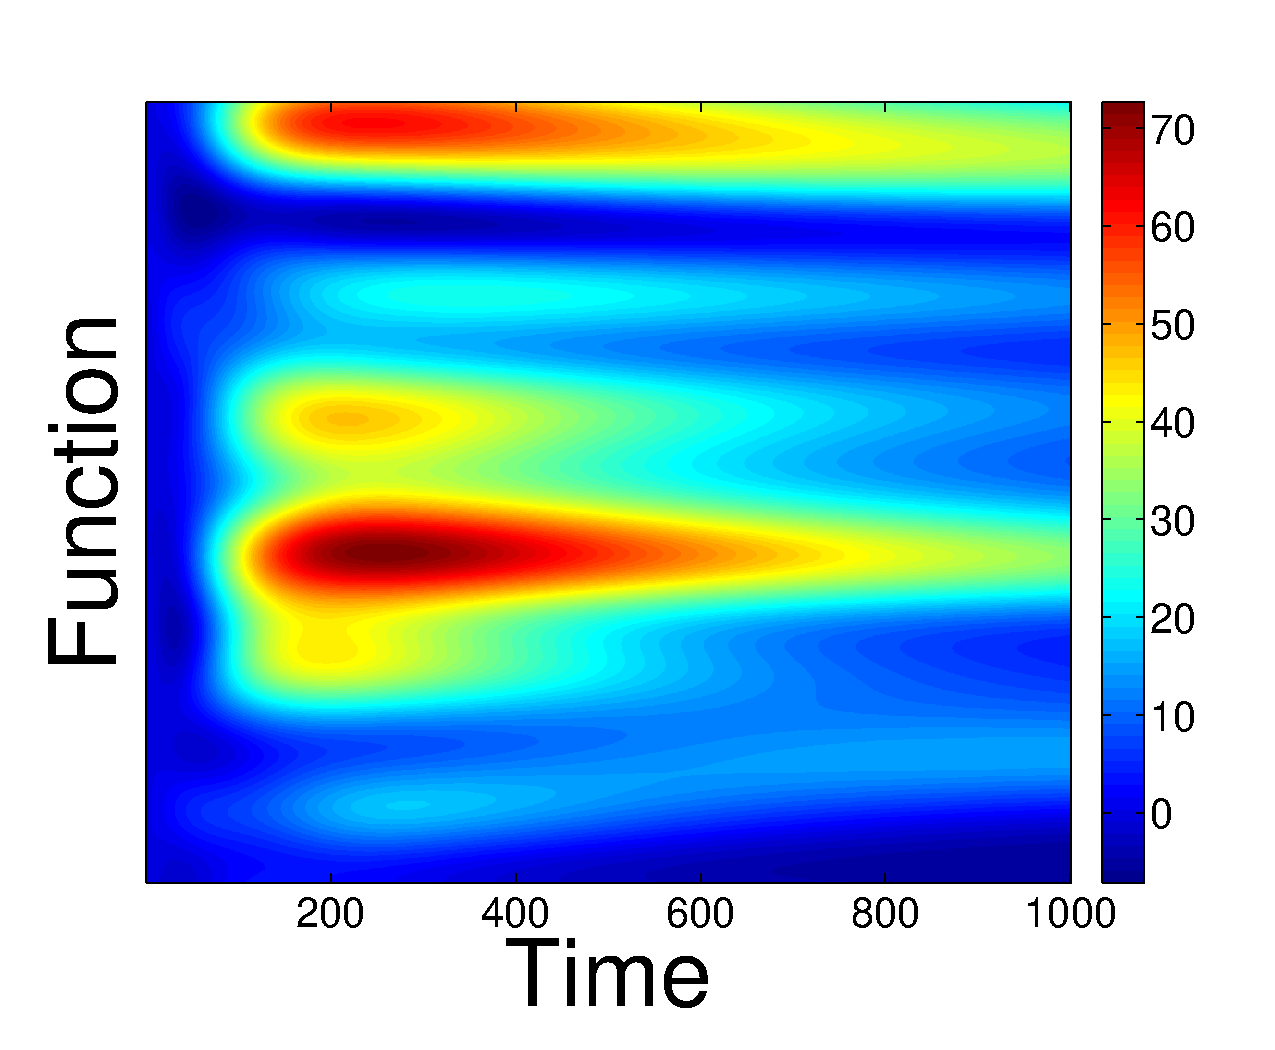
\includegraphics[width=0.25\columnwidth]{figures/kernel_evol_gaussian.pdf}
}
\subfloat[\small{Laplacian}]{
 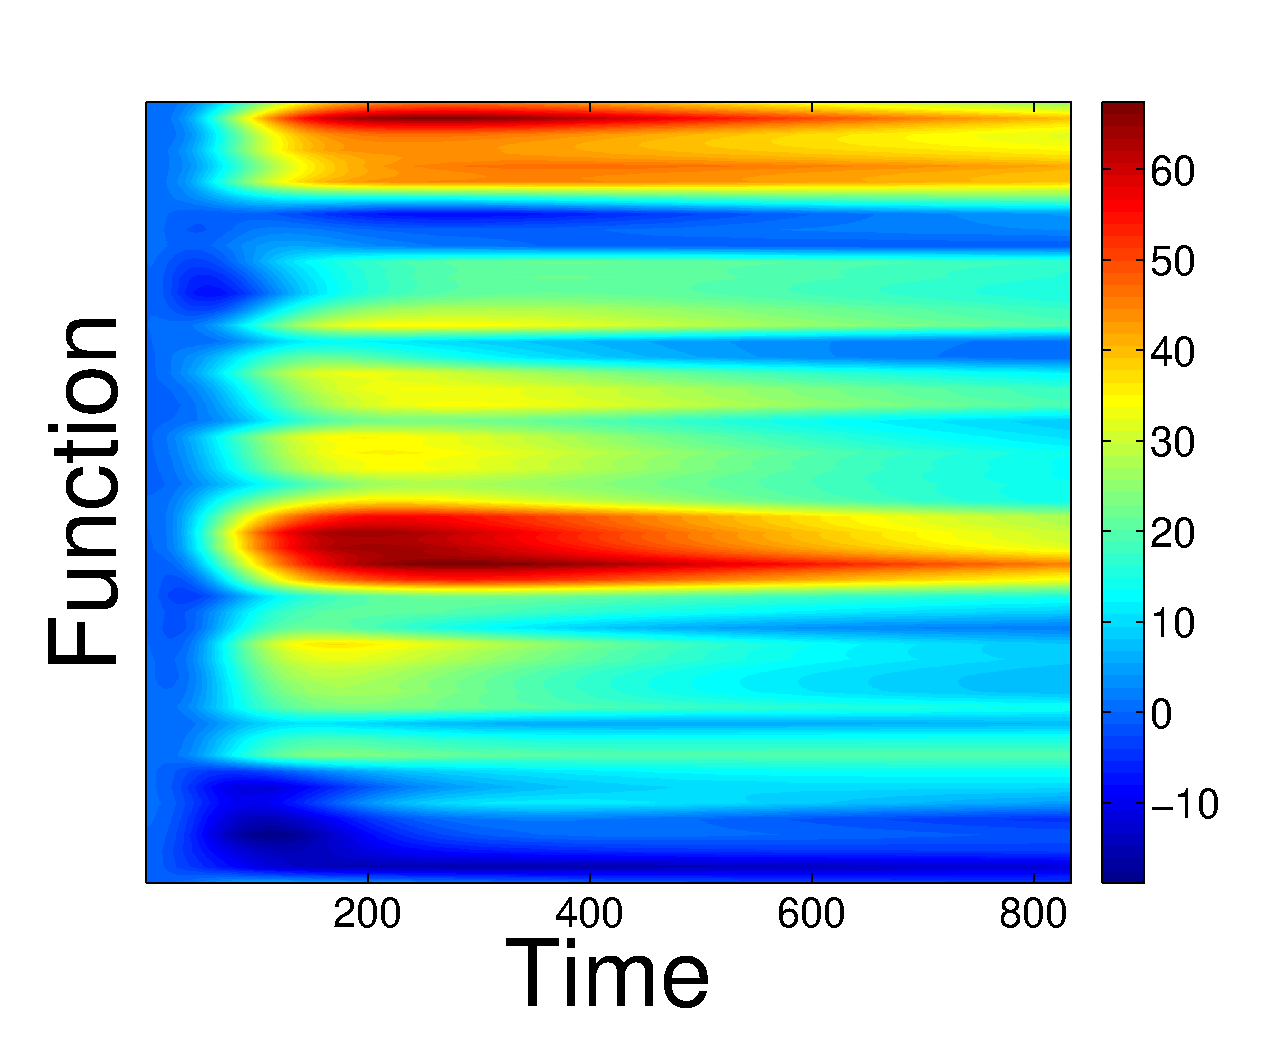
\includegraphics[width=0.25\columnwidth]{figures/kernel_evol_laplacian.pdf}
}
% \\
\subfloat[\small{Periodic}]{
 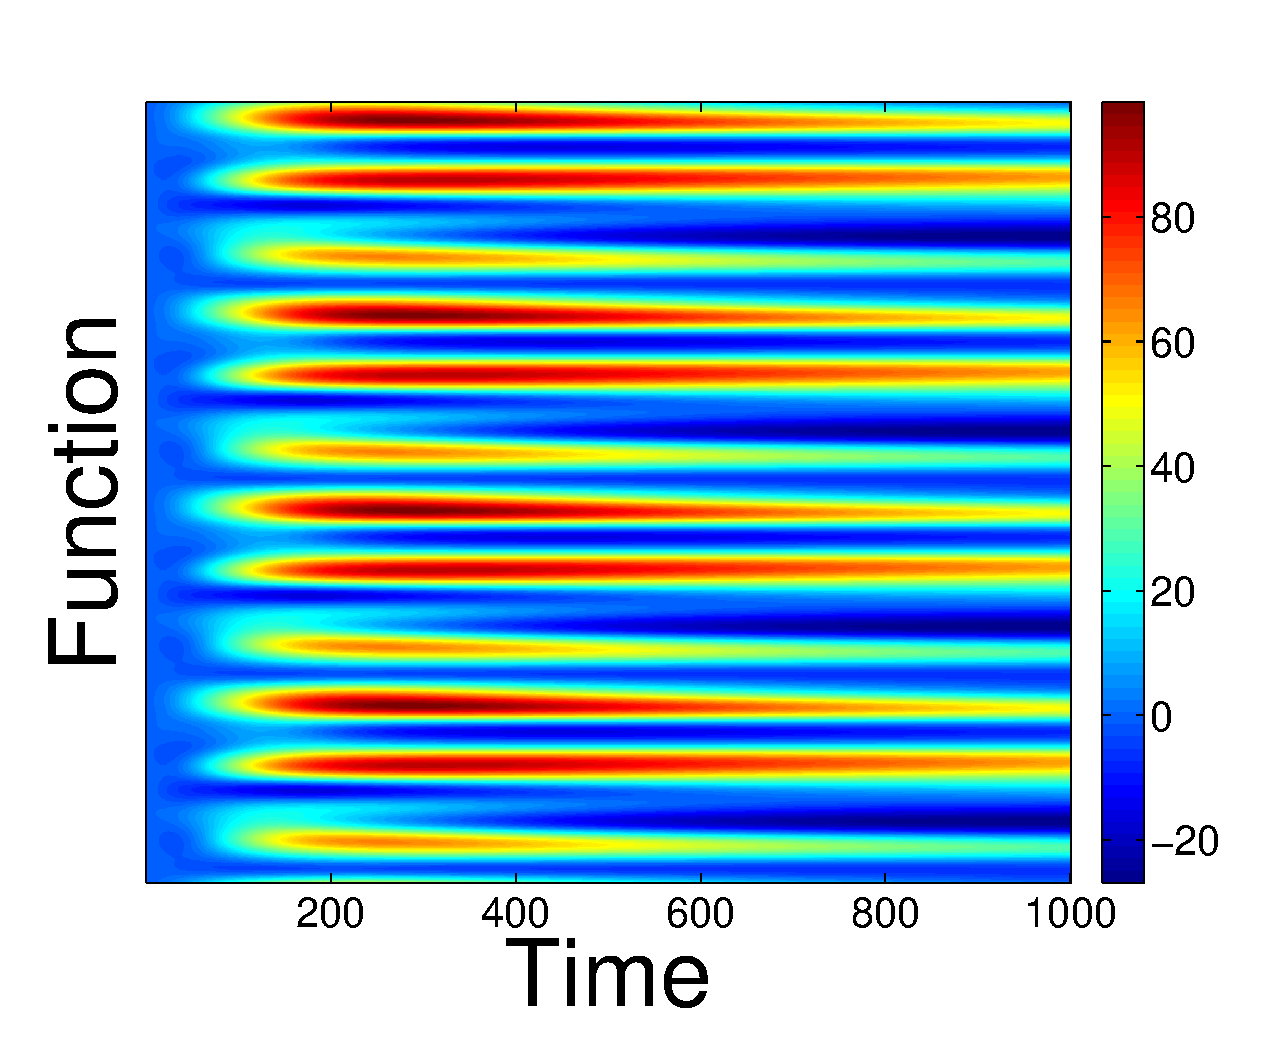
\includegraphics[width=0.25\columnwidth]{figures/kernel_evol_periodic.pdf}
}
% \subfloat[\small{Locally periodic}]{
%   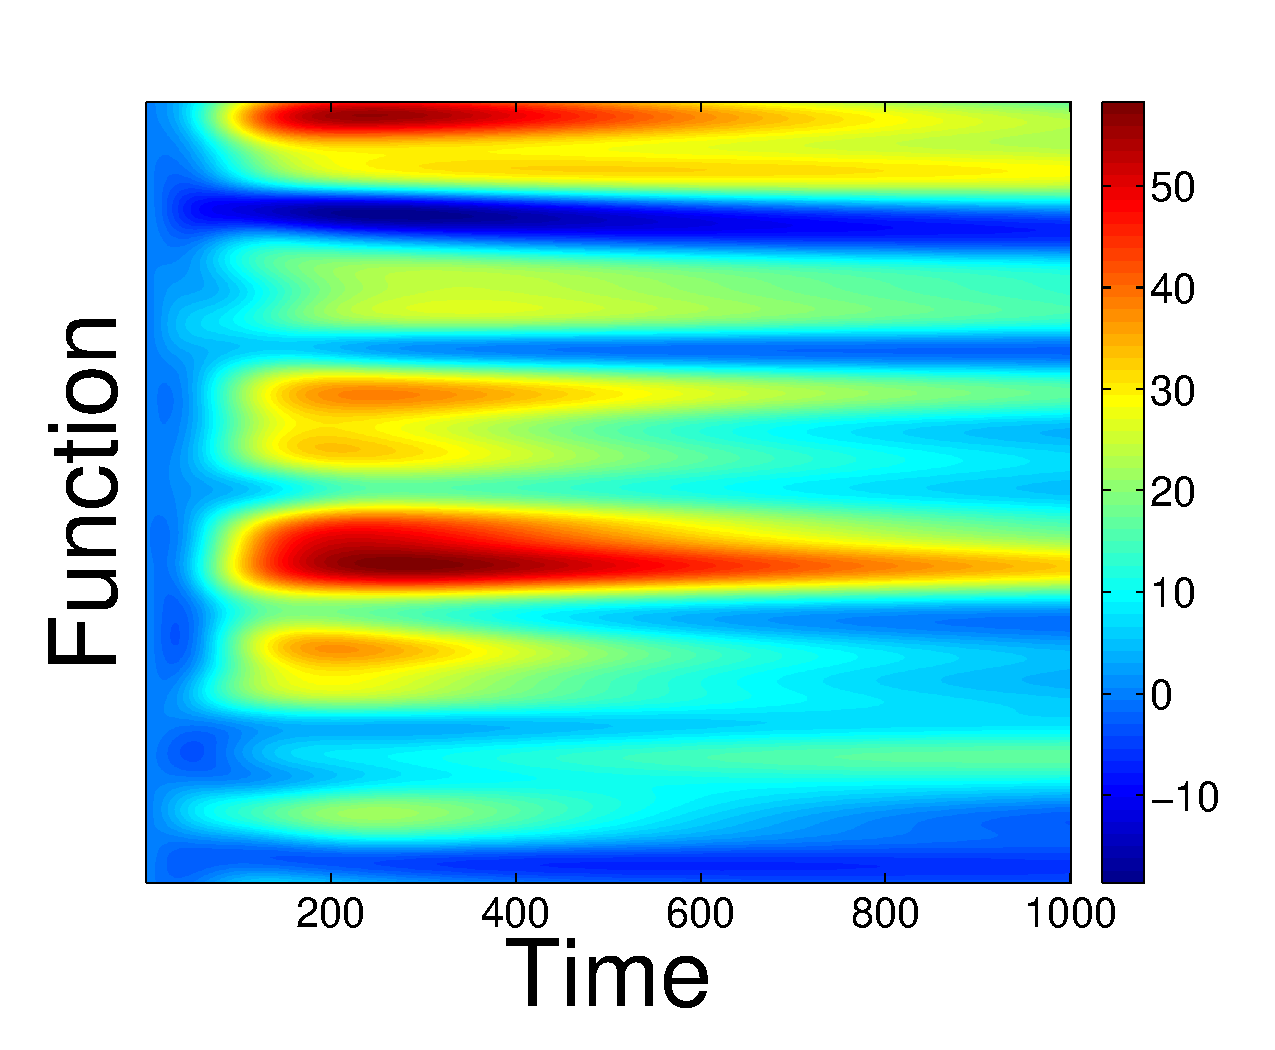
\includegraphics[width=0.3\columnwidth]{figures/kernel_evol_locally_periodic.pdf}
%}
\caption{\small{One-dimensional function evolution over a fixed transition matrix $A$, 
initial condition $\weight_0$ and centers $\shCent$, but with different kernels $\kernel(x,y)$. 
Each $y$-vector at a given value of $x$ represents the output of the function, which evolves from left to right. 
As seen, changing the kernel creates quite different dynamic behaviors. }%behavior for the same system.}
}
\label{fig:kernel_variation}
\end{figure}
In this paper, we restrict our attention to the class of functional evolutions $\mathbb{F}$ defined by linear Markovian transitions in an RKHS. While extension to the nonlinear case is possible (and non-trivial), it is not pursued in this paper to help ease the exposition of the key ideas. The class of linear transitions in RKHS is rich enough to approximately model many real-world datasets, as suggested by our experiments.

Let $y\in\R^{\nsamp}$ be the measurements of the function available from $\nsamp$ sensors, $\sysop:\fspace\to\fspace$ be a linear transition operator in the RKHS $\fspace$, and $\measop:\fspace\to\R^{\nsamp}$ be a linear measurement operator. The model for the functional evolution and measurement studied in this paper is:
\begin{align}\eqlabel{ideal_lin_evol}
 f_{\tindex+1} = \sysop f_{\tindex} + \eta_{\tindex}, \quad
 y_{\tindex} = \measop_{\tindex} f_{\tindex} + \zeta_{\tindex},
\end{align}
where $\eta_{\tindex}$ is a zero-mean stochastic process in $\fspace$, and $\zeta_{\tindex}$ is a Wiener process in $\R^{\nsamp}$. 
Classical treatments of kernel methods emphasize that for most kernels, the feature map $\fmap$ is unknown, and possibly infinite-dimensional; this forces practioners to work in the dual space of $\fspace$, whose dimensionality is the number of samples in the dataset being modeled. This conventional wisdom precludes the use of kernel methods for most tasks involving modern datasets, which may have millions and sometimes billions of samples \cite{rahimi2007random}. An alternative is to work with a feature map 
$\fmapApprox(x) := \left[\begin{smallmatrix}
  \fmapApprox_1(x) & \cdots & \fmapApprox_{\ncent}(x)
 \end{smallmatrix}\right]^T$ to an approximate feature space
 $\fspaceApprox$, with the property that for every element $\fspaceEl\in\fspace$, $\exists\fspaceApproxEl\in\fspaceApprox$ and an $\e >0$ s.t. $\|\fspaceEl-\fspaceApproxEl\| < \e$ for an appropriate function norm. A few such approximations are listed below.
%\begin{enumerate}
\paragraph{Dictionary of atoms} Let $\dom$ be compact. Given points $\shCent = \shCentLong$, $c_i\in\dom$, we have a dictionary of atoms $\Atoms = \{\fmap(c_1), \cdots , \fmap(c_{\ncent})\}$, $\fmap(c_i)\in\fspace$, the span of which is a strict subspace $\fspaceApprox$ of the RKHS $\fspace$ generated by the kernel. Here, 
 \begin{equation}\eqlabel{fmap_dict}
 \fmapApprox_i(x) := \l\fmap(x), \fmap(c_i)\r_{\fspace} = \kernel(x, c_i).
 \end{equation}
\paragraph{Low-rank approximations} Let $\dom$ be compact, let $\shCent = \shCentLong$, $c_i\in\dom$, and let $\empK\in\R^{\ncent\times\ncent}$, $\empK_{ij}:=\kernel(c_i,c_j)$ be the Gram matrix computed from $\shCent$. This matrix can be diagonalized to compute approximations $(\empEval_i, \empEfunc_i(x))$ of the eigenvalues and eigenfunctions $(\eval_i, \efunc_i(x))$ of the kernel \cite{williams2001using2}. These spectral quantities can then be used to compute  $ \fmapApprox_i(x):=\sqrt{\empEval}_i\empEfunc_i(x)$.
 \paragraph{Random Fourier features} Let $\dom\subset\R^n$ be compact, and let $ \kernel(x,y) = e^{-\|x-y\|^2/2\s^2}$ be the Gaussian RBF kernel. Then random Fourier features approximate the kernel feature map as $\fmapApprox_{\randFreq}:\dom\to\fspaceApprox$, where $\randFreq$ is a sample from the Fourier transform of $\kernel(x,y)$, with the property that $\kernel(x,y) = \E_{\randFreq}[\l\fmapApprox_{\randFreq}(x),\fmapApprox_{\randFreq}(y)\r_{\fspaceApprox}]$ \cite{rahimi2007random}. In this case, if $\randMat\in\R^{M/2\times n}$ is a random matrix representing the sample $\randFreq$, then 
 $ 
  \fmapApprox_i(x) := \left[\begin{smallmatrix}
  \frac{1}{\sqrt{\ncent}}\sin([\randMat x]_i), \frac{1}{\sqrt{\ncent}}\cos([\randMat x]_i)
 \end{smallmatrix}\right]$. Similar approximations exist for other radially symmetric kernels, as well as dot-product kernels. 

\begin{figure}
\centering
\subfloat[Relationship between $\sysop$ and $A$]{
\label{fig:commute_sysop_dyn}
%\resizebox{0.3\columnwidth}{0.06\paperheight}{%
\begin{tikzpicture}
  \matrix (m) [ampersand replacement=\&, matrix of math nodes, 
                 row sep=0.75in,column sep=1in,minimum width=0.5in] {
     \boldsymbol\fspaceApprox \& \boldsymbol\fspaceApprox \\
     \pmb{\R^{\ncent}} \& \pmb{\R^{\ncent}} \\};
  \path[-stealth]
    (m-1-1) edge node [left] {$\boldsymbol\weightmap$} (m-2-1)
            edge [right] node [above] {$\boldsymbol\sysop$} (m-1-2)
    (m-2-1.east|-m-2-2) edge node [below] {$\boldsymbol A$} node [above] {} (m-2-2)
    (m-2-2) edge node [right] {$\boldsymbol\weightmapI$} (m-1-2);            
\end{tikzpicture}  
%}% end resize box
}% end subfloat
\
\subfloat[Relationship between $\measop$ and $\empK$]{
\label{fig:commute_sysop_meas}
%\resizebox{0.3\columnwidth}{0.06\paperheight}{%
\begin{tikzpicture}
  \matrix (m) [ampersand replacement=\&, matrix of math nodes, 
               row sep=0.75in,column sep=1in,minimum width=0.5in] {
     \boldsymbol\fspaceApprox \& \pmb{\boldsymbol\R^{\nsamp}} \\
     \pmb{\R^{\ncent}} \&  \\};
  \path[-stealth]
    (m-1-1) edge node [left] {$\boldsymbol\weightmap$} (m-2-1)
            edge [right] node [above] {$\boldsymbol\measop$} (m-1-2)
    (m-2-1) edge node [right] {$\ \boldsymbol\empK$} (m-1-2)
    (m-2-1) edge node [right] {$\boldsymbol\weightmapI$} (m-1-1);            
\end{tikzpicture}
%}% end resize box
}% end subfloat
\
\subfloat[Relationship between $\controlop$ and $B$]{
\label{fig:commute_sysop_control}
%\resizebox{0.3\columnwidth}{0.06\paperheight}{%
\begin{tikzpicture}
  \matrix (m) [ampersand replacement=\&, matrix of math nodes, 
                 row sep=0.75in,column sep=1in,minimum width=0.5in] {
     \boldsymbol\fspaceD \& \boldsymbol\fspaceApprox \\
     \pmb{\R^{\ncontrol}} \& \pmb{\R^{\ncent}} \\};
  \path[-stealth]
    (m-1-1) edge node [left] {$\boldsymbol\weightmapC$} (m-2-1)
            edge [right] node [above] {$\boldsymbol\controlop$} (m-1-2)
    (m-2-1.east|-m-2-2) edge node [below] {$\boldsymbol B$} node [above] {} (m-2-2)
    (m-2-2) edge node [right] {$\boldsymbol\weightmapI$} (m-1-2);            
\end{tikzpicture}
%}% end resize box
}% end subfloat
\caption{Commutative diagrams between primal and dual spaces}
\vspace{-0.2in}
\label{fig:commute_sysop}
\end{figure}
%\end{enumerate}
In the approximate space case, we replace the transition operator $\sysop:\fspace\to\fspace$ in \eqref{ideal_lin_evol} by $\sysopApprox:\fspaceApprox\to\fspaceApprox$.
This approximate regime, which combines the flexibility of a truly nonparametric approach with computational realizability, still allows for the representation of rich phenomena, as will be seen in the sequel, and in Figure \ref{fig:kernel_variation}. 
The finite-dimensional evolution equations approximating \eqref{ideal_lin_evol} in dual form are
\vspace{-0.05in}
\begin{align} \eqlabel{k_measure}
 \weight_{\tindex+1} = \dualopApprox\weight_{\tindex} + \processnoise_{\tindex}, \quad 
 \meas_{\tindex} = \obsMat \weight_{\tindex} +\measnoise_{\tindex},
\end{align}
where we have matrices $\dualopApprox\in \R^{\ncent\times\ncent}, \ \obsMat\in \R^{\nsamp\times\ncent}$, the vectors $\weight_{\tindex}\in\R^{\ncent}$, and where we have slightly abused notation to let $\meas_{\tindex}, \processnoise_{\tindex}$ and $\measnoise_{\tindex}$ denote their $\fspaceApprox$ counterparts. Here $\obsMat$ is the matrix whose rows are of the form $\obsMat_{(i)} = \obsMatRow(x_i) =
 \left[\begin{smallmatrix}
  \fmapApprox_1(x_i) & \fmapApprox_2(x_i) & \cdots & \fmapApprox_{\ncent}(x_i)
 \end{smallmatrix}\right]$. In systems-theoretic language, each row of $\obsMat$ corresponds to a \emph{measurement} at a particular location, and the matrix itself acts as a measurement operator. 

The equations \eqref{ideal_lin_evol} suggest an immediate extension to functional control problems. 
Pick another basis for $\fspace$ as $\cbasis(x) := \begin{bmatrix}\cbasis_1(x) &\cdots & \cbasis_{\ncontrol}(x)
\end{bmatrix}^T$, where the functions $\cbasis_j(x)$ are used to approximate the RKHS $\fspace$ generated by the kernel. We denote the span of these functions as $\fspaceD$. In the dictionary of atoms case, an example would be another set of atoms
 $\AtomsControl = \begin{bmatrix}\fmap(d_1) &\cdots & \fmap(d_{\ncontrol})
\end{bmatrix}$, $\fmap(d_j)\in\fspace$, $d_j\in\dom$, with $\fspaceD$ being a strict subspace of the RKHS $\fspace$  generated by the kernel. 
The functional evolution equation is then as follows:
\begin{align}\eqlabel{ideal_lin_evol_control}
 f_{\tindex+1} = \sysop f_{\tindex} + \controlop \control_{\tindex} + \eta_{\tindex}, \quad y_{\tindex} = \measop_{\tindex} f_{\tindex} + \zeta_{\tindex},
\end{align}
where the control functions $\control_{\tindex}$ evolve in $\fspaceD$, and $\controlop:\fspaceD\to\fspaceApprox$. To derive the finite-dimensional equivalent of $\controlop$, we have to work out the structure of the matrix $B$: since $\fspaceApprox$ is not, in general, isomorphic to $\fspaceD$, this imposes strict restrictions on $B$. We can derive $B$ using least squares using the inner product of $\fspace$. An instructive example is where both $\fspaceApprox$ and $\fspaceD$ are generated by dictionaries of atoms; recall that in this case, $\Atoms = 
 \begin{bmatrix}\fmap(c_1) &\cdots & \fmap(c_{\ncent})
\end{bmatrix}$ is the basis for $\fspaceApprox$, and let $\control = \sum_{j=1}^{\ncontrol}\weightc_j\fmap(d_j)$, and let $\Atoms = 
 \begin{bmatrix}\fmap(c_1) &\cdots & \fmap(c_{\ncent})
\end{bmatrix}$ be the basis for $\fspaceC$. Then the projection of $\delta$ onto $\fspaceApprox$ can be derived as 
%\begin{align*}
%\vspace{0.1in}
\resizebox{1.0\columnwidth}{!}{ 
 $\begin{bmatrix}
  \l \delta, \fmap(c_1) \r_{\fspace}\\
   \vdots\\
  \l \delta, \fmap(c_{\ncent}) \r_{\fspace} 
 \end{bmatrix}
 = 
 \underbrace{
 \begin{bmatrix}
  \Kiprod{d_1}{c_1} & \cdots & \Kiprod{d_{\ncontrol}}{c_1}\\
   \vdots  &\ddots &\vdots\\
  \Kiprod{d_1}{c_{\ncent}} & \cdots & \Kiprod{d_{\ncontrol}}{c_{\ncent}}
 \end{bmatrix}}_{\empKCD}
  \begin{bmatrix}
   \weightc_1\\
   \vdots\\
   \weightc_{\ncontrol}
  \end{bmatrix}.$
}
%\end{align*}
Note that in the dictionary of atoms case, the entries of $\empKCD$ can be computed in closed form as ${\empKCD}_{ij}:= \kernel(d_i, c_j)$,
using the reproducing property. 
This derivation shows that the operator $B$ is simply $\empKCD\in\R^{\ncent\times\ncontrol}$, the kernel matrix between the data $\centers$ generating the atoms $\Atoms$ of $\fspaceApprox$ and the data $\centerscontrol$ generating the atoms $\AtomsControl$ of $\fspaceD$. 
% Using similar arguments, it can be shown that, given sensing locations $\data = \{x_1,x_2,\dots, x_{\nsamp}\}$, $\empKD\in\R^{\nsamp\times\ncontrol}$ is the kernel matrix between $\data$ and $\centerscontrol$. 
Thus, the finite-dimensional evolution equations equivalent to \eqref{ideal_lin_evol_control} are
\begin{align}
 \weight_{\tindex} = \dualopApprox\weight_{\tindex} + \empKCD\weightc_{\tindex}, \quad
 y_{\tindex} = \empK_{\tindex} w_{\tindex} \eqlabel{k_measure_c1}.
\end{align}
We define the \emph{generalized observability matrix} \cite{zhou:bk:96} as 
%\begin{align}\eqlabel{obs_mat}
$  \Obs_{\Tset} = 
 \left[
 \begin{smallmatrix}
  \empK \dualopApprox^{\tindex_1}\\
  \cdots\\
  \empK \dualopApprox^{\tindex_\otime}
 \end{smallmatrix}
 \right] $
%\end{align}
where $\Tset = \{\tindex_1, \dots, \tindex_{\otime}\}$ are the set of instances $\tindex_i$
when we apply the operator $\empK$. A linear system is said to be \emph{observable} if $\Obs_{\Tset}$ has full column rank (i.e. $\mathrm{Rank} (\Obs_{\Tset})=\ncent$) for 
$\Tset = \{0, 1, \dots, \ncent-1\}$ \cite{zhou:bk:96}. Observability guarantees two critical facts: firstly, it guarantees that the state $\weight_0$ can be recovered exactly from a finite series of measurements $\{y_{{\tindex}_1}, y_{{\tindex}_2}, \dots, y_{{\tindex}_{\otime}}\}$; in particular, defining $y_{\Tset} = \begin{bmatrix}y_{{\tindex}_1}^T, y_{{\tindex}_2}^T, \cdots, y_{{\tindex}_{\otime}^T}\end{bmatrix}^T$, we have that $y_{\Tset} = \Obs_{\Tset}\weight_0.$  Secondly, it guarantees that a feedback based \emph{observer} can be designed such that the estimate of $\weight_{\tindex}$, denoted by $\estweight_{\tindex}$, converges exponentially fast to $\weight_{\tindex}$ in the limit of samples. Note that all our theoretical results assume $\dualopApprox$ is available: while we perform system identification in the experiments (\cite{Kingravi16_NIPS}), it is not the focus of the paper. 

We are now in a position to formally state the spatiotemporal modeling, control, and inference problems being considered: given a spatiotemporally evolving system modeled using \eqref{k_measure}, choose a set of $\nsamp$ sensing locations such that even with $\nsamp\ll \ncent$, the functional evolution of the spatiotemporal model can be estimated (which corresponds to \emph{monitoring}), can be predicted robustly (which corresponds to \emph{Bayesian filtering}), and which can be controlled (which corresponds to \emph{functional control}). Our approach to solve the monitoring and prediction problem relies on the design of the measurement operator $\empK$ so that the pair $(\empK, \dualopApprox)$ is observable: any Bayesian state estimator (e.g. a Kalman filter) utilizing this pair is denoted as a \textbf{kernel observer} \footnote{In the case where no measurements are taken, for the sake of consistency, we denote the state estimator as an \textbf{autonomous kernel observer}, despite this being somewhat of an oxymoron.}. In the controls case, given a spatiotemporally evolving system modeled using \eqref{k_measure_c1}, we need to choose a set of $\nsamp$ sensing locations and $\ncontrol$ control locations, such that even with $\nsamp\ll \ncent, \ \ncontrol \ll\ncent$, the functional evolution of the spatiotemporal model can be controlled; in this case, we must design both a measurement operator $\empK$ and a control operator $\empKCD$ such that the pair $(\empKCD, \dualopApprox)$ is controllable: a controls system utilizing this pair and the measurement operator $\empK$ is denoted as a \textbf{kernel controller}.

\subsection{Preliminaries on Rational Canonical Structures}\label{sec_prelim}
We take a geometric approach towards the choice of sampling locations for inferring $\weight_{\tindex}$ in  \eqref{k_measure}; the extension for control is similar.  We use the notation $\linspace$, with $\dims(\linspace)=\ncent$, to emphasize the fact that these theorems hold for any finite-dimensional vector space. Consider the linear operator $\sysop:\linspace\rightarrow\linspace$, and recall that the definition of observability requires the construction of a linear operator $\measop:\linspace\to\linspaceout$, with $\dim(\linspaceout) = \nsamp$, such that 
$\Rank\left[
 \begin{smallmatrix}
  \left(\measop\right)^T &
  \cdots &
  \left(\measop \sysop^{\ncent-1}\right)^T
 \end{smallmatrix}
 \right]^T = \ncent$. 
In most applications, if $\nsamp\geq\ncent$, and $\Rank\measop = \nsamp$, it is reasonable to expect that observability may be achieved. However, for our purposes, $\nsamp$ must be \emph{significantly} less than $\ncent$. Therefore, we must design $\measop$ with as small a rank as possible. To do so, we require a series of vectors $\linvec_i$ that, under repeated iterations of $\sysop$, can generate a basis for $\linspace$. For this task, we will use a fundamental decomposition result from the theory of modules, known as the \emph{rational canonical structure} of $\sysop$ \cite{wonham1974linear}. The intuition here is that if the sequence $\{\linvec_i\}_{i}$ can generate this basis, it can be directly used to construct $\measop$.

The linear operator $\sysop:\linspace\rightarrow\linspace$ has a characteristic polynomial $\charpoly(\eval) $ such that $\charpoly(\sysop)=0 $ by the Cayley-Hamilton theorem. The minimal polynomial (MP) of $\sysop$ is the monic polynomial $\minpoly(\cdot)$ of least degree (denoted by $\degs(\cdot)$) given as 
$\minpoly(\eval) = \polycoeff_0 + \polycoeff_1\eval +\cdots + \eval^{\degs(\minpoly)} = 0$, such that
$\minpoly(\sysop)=\polycoeff_0 I + \polycoeff_1\sysop +\cdots + \sysop^{\degs(\minpoly)} = \bm{0}$. 
The MP is unique and divides $\charpoly(\lambda)$, so that $ \degs(\minpoly) \leq \degs(\charpoly)$. The MP of a vector $\linvec\in\linspace$ \emph{relative to $\sysop$} is the unique monic polynomial $\minpolyv_{\linvec}$ of least degree such that 
$\minpolyv_{\linvec}(\sysop)\linvec= \polycoeff_0\linvec + \polycoeff_1\sysop\linvec + \cdots + \sysop^{\degs(\minpoly)}\linvec = 0$. 
If $\degs(\alpha) = \ncent$, then $\sysop$ is \emph{cyclic} and $\exists\linvec\in \linspace$, such that the vectors $\{\linvec, \sysop \linvec,\dots,\sysop^{\ncent-1}\linvec\}$ form a basis for $\linspace$; this is the same as saying that the pair $(\linvec^T,\sysop^T)$ is observable.    
A subspace $\subspace\subset\linspace$ s.t. $\sysop\subspace\subset\subspace$ is \emph{$\sysop$-cyclic} if  $\restrict{\sysop}{\subspace}$, the restriction of $\sysop$ to the subspace $\subspace$, is cyclic. If $\minpoly(\eval)$ is the minimal polynomial of $\sysop$ and $\degs(\minpoly) = \acycdeg < \ncent$, $\exists~\linvec\in\linspace$ such that $\{\linvec, \sysop \linvec,\dots,\sysop^{\acycdeg-1}\linvec\}$ span an $\acycdeg$-dimensional $\sysop$-cyclic subspace $\subspace$, with $\linvec$ being the \emph{cyclic generator} of $\subspace$.  The subspace $\subspace$ decomposes $\linspace$ relative to $\sysop$. By the rational canonical structure theorem (Theorem 0.1 of \cite{wonham1974linear}), $\sysop$ can be successively decomposed into subspaces $\linspace_i \subset \linspace$, $i\in \{1,\dots,\minmeas\}$, s.t. $\linspace = \linspace_1 \oplus ... \oplus \linspace_{\minmeas}$, $\sysop\linspace_i \subset \linspace_i$, and  $\sysop_{|\linspace_i}, i \in \{1,\dots,\minmeas\}$, are cyclic\footnote{In general, the subspaces $\linspace_i$ are not unique for a fixed $\sysop$.}. The integer $\minmeas$ is unique and is called the \emph{cyclic index of $\sysop$}. 

One of our main results is to show that the cyclic index is a lower bound on the number of measurements required to reconstruct $\weight_{\tindex}$ (see Prop. \ref{prop:3} and Alg. 1 in \cite{Kingravi16_NIPS}). The matrix transform associated to this theorem is known as the \emph{Frobenius normal form} (denoted by $\FrobC\in\R^{\ncent\times\ncent}$ ): for $\sysop\in\R^{\ncent\times\ncent}$,  $\exists \FrobP\in\R^{\ncent\times\ncent}$ invertible  such that $\sysop = \FrobP\FrobC\FrobP^{-1}$. We will also use the \emph{Jordan decomposition}, where for $\sysop\in\R^{\ncent\times\ncent}$, $\exists \JorP\in\R^{\ncent\times\ncent}$ invertible such that $\sysop = \JorP\JorLa \JorP^{-1}$, where $\JorLa$ is a unique block diagonal matrix with Jordan blocks with $\eval_i$ along the diagonal. 
If all the eigenvalues $\eval_i$ are nonzero and real, we say the matrix has a \emph{full-rank Jordan decomposition}. 


\vspace{-0.1in}




\subsection{Main Results}\label{sec:theory_results}
%\vspace{-0.1in}
In this section, we prove results concerning the observability of spatiotemporally varying functions modeled by the functional evolution and measurement equations \eqref{k_measure}. In particular,  observability of the system states implies that we can recover the current state of the spatiotemporally varying function using a small number of sampling locations $\nsamp$, which allows us to 1) track the function, and 2) predict its evolution forward in time. We work with the approximation $\fspaceApprox\approx\fspace$: given $\ncent$ basis functions, this implies that the dual space of $\fspaceApprox$ is $\R^{\ncent}$.
Proposition \ref{prop:1} shows that if $\dualopApprox$ has a full-rank Jordan decomposition, the observation matrix $\obsMat$ meeting a condition called \emph{shadedness} (Definition \ref{def:shaded}) is sufficient for the system to be observable. Proposition \ref{prop:2} provides a lower bound on the number of sampling locations required for observability which holds for any $\dualopApprox$.  Proposition \ref{prop:3} constructively shows the existence of an abstract measurement map $\measmap$ achieving this lower bound. Since the measurement map does not have the structure of a kernel matrix, a slightly weaker sufficient condition for the observability of any $\dualopApprox$ is in Theorem \ref{thm:1}. Finally, since both $\empK$ and $\empKCD$ are kernel matrices generated from a shared kernel, these observability results translate directly into controllability results. Proofs of all claims are in the appendix. 

\begin{definition}\label{def:shaded}
\textbf{(Shaded Observation Matrix)} Given $\kernel:\dom\times\dom\to\R$ positive-definite on a domain $\dom$, let $\{\fmapApprox_1(x), \dots, \fmapApprox_{\ncent}(x)\}$ be the set of bases generating an approximate feature map $\fmapApprox:\dom\to\fspaceApprox$, and let
$\sampSet = \sampSetLong$ be the set of sampling (or sensing) locations, with each $x_i\in\dom$. 
Let $\obsMat\in\R^{\nsamp\times\ncent}$ be the observation matrix, where $ \obsMat_{ij} := \fmapApprox_j(x_i)$. For each
row $\obsMat_{(i)} := \left[\begin{smallmatrix}
  \fmapApprox_1(x_i) & \cdots & \fmapApprox_{\ncent}(x_i)
 \end{smallmatrix}\right]$, define the set 
$\Ind_{(i)} := \{\iota_1^{(i)},\iota_2^{(i)},\dots, \iota_{\ncent_i}^{(i)}\}$ to be the indices in the observation
matrix row $i$ which are nonzero. 
Then if 
%\begin{align}\eqlabel{shaded_cond}
$\bigcup_{i\in\{1,\dots,\nsamp\}} \Ind^{(i)} = \{1,2,\dots, \ncent\}$,
%\end{align}
we denote $\obsMat$ as a \emph{shaded observation matrix} (see Figure \ref{fig:shadeda}).
\end{definition}

This definition seems quite abstract, so the following remark considers a more concrete example.

\begin{remark}\label{rem:shaded}
 let $\fmapApprox$ be generated by the dictionary given by $\shCent = \shCentLong$, $c_i\in\dom$. Note that since $\fmapApprox_j(x_i) = \l\fmap(x_i), \fmap(c_j)\r_{\fspace} = \kernel(x_i,c_j)$, $\obsMat$ is the kernel matrix between $\sampSet$ and $\shCent$. For the kernel matrix to be shaded thus implies that there does not exist an atom $\fmap(c_j)$ such that the projections $\l\fmap(x_i),\fmap(c_j)\r_{\fspace}$ vanish for all $x_i$, $1\leq i\leq \nsamp$. Intuitively, the shadedness property requires that the sensor locations $x_i$ are privy to information propagating from every $c_j$. As an example, note that, in principle, for the Gaussian kernel, a single row generates a shaded kernel matrix. However, in this case, the matrix can have many entries that are extremely close to zero, and will probably be very ill-conditioned.  
\end{remark}

% With this definition in place, we can prove the following proposition, which shows that if $\dualopC$ has a full-rank Jordan decomposition, a shaded observationrf matrix is sufficient to guarantee observability. 

\begin{proposition}\label{prop:1}
Given $\kernel:\dom\times\dom\to\R$ positive-definite on a domain $\dom$, let $\{\fmapApprox_1(x), \dots, \fmapApprox_{\ncent}(x)\}$ be the set of bases generating an approximate feature map $\fmapApprox:\dom\to\fspaceApprox$, and let
$\sampSet = \sampSetLong$, $x_i\in\dom$. Consider the discrete linear system on $\fspaceApprox$ given by the evolution and measurement equations \eqref{k_measure}. Suppose that a full-rank Jordan decomposition of $\dualopApprox\in\R^{\ncent\times\ncent}$ of the form $\dualopApprox = \JorP\JorLa\JorP^{-1}$ exists, where $\JorLa = 
\left[\begin{smallmatrix}\JorLa_1 &\cdots & \JorLa_{\JorMul}\end{smallmatrix}\right]$,
and there are no repeated eigenvalues. Then, given a set of time instances  $\Tset = \{\tindex_1,\tindex_2,\dots,\tindex_{\otime}\}$, and a set of sampling locations $\sampSet=\sampSetLong$,
the system \eqref{k_measure} is observable if the observation matrix $\empK_{ij}$ is shaded according to Definition \ref{def:shaded},
% $\empK^D$, the row vector generated by summing the rows of $\empK$, has all nonzero entries, 
$\Tset$ has distinct values, and $|\Tset| \geq \ncent$.
\end{proposition}

% \begin{remark}
%  For the system corresponding to \ref{prop:1}, 
% \end{remark}
When the eigenvalues of the system matrix are repeated, it is not enough for $\empK$ to be shaded. 
% Intuitively, repeated eigenvalues correspond to coupled evolution\footnote{We use the term coupled evolution to denote dynamic evolution in which some eigen-modes evolve together \gXX{check rewrite}}, which requires an increased number of sensors to discern \gXX{what's the best way to explain this better? Without invariant subspaces it may not be clear to some why this matters, should we merge this with the discussion after the below prop?}. 
In the next proposition, we take a geometric approach and utilize the rational canonical form  of $\dualopApprox$ to obtain a lower bound on the number of sampling locations required. Let $\nevals$ be the number of unique eigenvalues of $\dualopApprox$, and let $\geomMult{\eval_i}$ denote the geometric multiplicity of eigenvalue $\eval_i$. Then the \emph{cyclic index} of $\dualopApprox$ is defined as $\minmeas = \max_{1\leq i\leq\nevals}{\geomMult{\eval_i}}$\cite{wonham1974linear}.

\begin{proposition}\label{prop:2}
 Suppose that the conditions in Proposition \ref{prop:1} hold, with the relaxation that
 the Jordan blocks $\left[\begin{smallmatrix}
                           \JorLa_1 &\cdots & \JorLa_{\JorMul}
                          \end{smallmatrix}\right]$ may have 
 repeated eigenvalues (i.e. $\exists \JorLa_i$ and $\JorLa_j$ s.t. $\eval_i = \eval_j$). 
 Then there exist kernels $\kernel(x,y)$ such that 
 the lower bound $\minmeas$ on the number of sampling locations $\nsamp$ is given by the cyclic index of $\dualopApprox$. In other words, the system in \eqref{k_measure} is observable if $ \nsamp \geq \ell$.
\end{proposition}

We will give a concrete example to build intuition regarding this lower bound below. For now, we note the following:
\begin{figure}[t!]
	\begin{algorithm}[H]
		\caption{Measurement Map $\measmap$}
		\label{alg:measmap}
		\begin{algorithmic}
				\STATE {\bfseries Input:} $\dualopApprox\in\R^{\ncent\times\ncent}$
				\STATE Compute Rational Canonical Form, s.t. $\FrobC = \FrobP^{-1}\dualopApprox^T\FrobP$. Set $\FrobC_0:=\FrobC$, and
				$\ncent_0:=\ncent$. 
				\FOR{$i=1$ {\bfseries to} $\minmeas$}
				\STATE Obtain MP $\minpoly_i(\eval)$ of $\FrobC_{i-1}$. 
				This returns associated indices $\mmapInd{i}\subset\{1,2,\dots,\ncent_{i-1}\}$. 
				\STATE Construct vector $\linvec_i \in \R^{\ncent}$ such that 
				$\minpolyv_{\linvec_i}(\eval)=\minpoly_{i}(\eval)$ .
				\STATE Use indices $\{1,2,\dots,\ncent_{i-1}\}\setminus\mmapInd{i}$ to select matrix $\FrobC_i$. Set 
				$\ncent_i:= |\{1,2,\dots,\ncent_{i-1}\}\setminus\mmapInd{i}|$
				\ENDFOR
				\STATE Compute $ \premeasmap = [\linvec_1^T, \linvec_2^T,...,\linvec_{\minmeas}^T]^T$
				\STATE {\bfseries Output:} $\measmap =\premeasmap\FrobP^{-1}$
		\end{algorithmic}
	\end{algorithm}
\end{figure}
\begin{proposition}\label{prop:3}
Given the conditions stated in Proposition \ref{prop:2}, it is possible to construct a measurement map $\measmap \in \R^{\minmeas\times\ncent}$ for the system given by \eqref{k_measure}, such that the pair $(\measmap, \dualopApprox)$ is observable.
\end{proposition}

The construction provided in the proof of Proposition \ref{prop:3} is utilized in Algorithm 1, which uses the rational canonical structure of $\dualopApprox$ to generate a series of vectors $\linvec_i\in\R^{\ncent}$, whose iterations $\{\linvec_1,\dots,\dualopApprox^{\acycdeg_1-1}\linvec_1,\dots,\linvec_{\minmeas},\dots,\dualopApprox^{\acycdeg_{\minmeas}-1}\linvec_{\minmeas}\}$ generate a basis for $\R^{\ncent}$.
Unfortunately, the measurement map $\measmap$, being an abstract construction unrelated to the kernel, does not directly select $\sampSet$. We will show how to use the measurement map to guide a search for $\sampSet$ in Remark \ref{rem:1} (in Appendix). For now, we state a sufficient condition for observability of a general system. 

\begin{theorem}\label{thm:1}
 Suppose that the conditions in Proposition \ref{prop:1} hold, with the relaxation that
 the Jordan blocks $\begin{bmatrix}\JorLa_1 & &\cdots & \JorLa_{\JorMul}\end{bmatrix}$ may have 
 repeated eigenvalues. Let $\minmeas$ be the cyclic index of $\dualopApprox$.
 Define 
 \begin{align}\eqlabel{empKShadFull}
  \empKShadFull = \left[\begin{smallmatrix}
                    \empK^{{(1)}^T} & 
                    \cdots &
                    \empK^{{(\minmeas)}^T}
                  \end{smallmatrix}\right]^T
 \end{align}
 as the \emph{$\minmeas$-shaded matrix} (see Figure \ref{fig:shadedb}) which consists of $\minmeas$ shaded matrices with the property that any subset of
 $\minmeas$
 columns in the matrix are linearly independent from each
 other. Then system \eqref{k_measure} is observable if $\Tset$ has distinct values, and $|\Tset| \geq \ncent$.
\end{theorem}

While Theorem \ref{thm:1} is a quite general result, the condition that any $\minmeas$ columns of $\empKShadFull$ be linearly independent is a very stringent condition. 
One scenario where this condition can be met with minimal measurements is in the case when the feature map $\fmapApprox(x)$ is generated by a dictionary of atoms with the Gaussian RBF kernel evaluated at sampling locations $\sampSetLong$ according to \eqref{fmap_dict}, where $x_i\in\dom\subset\R^d$, and $x_i$ are sampled from a non-degenerate probability distribution on $\dom$ such as the uniform distribution. For a semi-deterministic approach, when the dynamics matrix $\dualopApprox$ is block-diagonal, we can utilize a simple heuristic:

\begin{remark}\label{rem:1}
 Let $\dom$ be compact, $\shCent = \shCentLong$, $c_i\in\dom$, and let the approximate feature map be defined by \eqref{fmap_dict}. Consider the system \eqref{k_measure} with $\dualopApprox=\JorLa$, and let $\Tset = \{0,1,\dots,\ncent-1\}$. Then the measurement map $\measmap$'s values lie in $\{0, 1\}$; in particular, each row $\measmap^{(j)}$, $j\in\{1,\dots,\minmeas\}$, corresponds to a subspace $\fsubspaceC{j}$, generated by a subset of centers $\shCent^{(j)}\subset\shCent$. Generate samples $x_i^{(j)}$ to create a kernel matrix $\empK^{(j)}$ that is shaded only with respect to centers $\shCent^{(j)}$. Once this is done, move on to the next subspace $\fsubspaceC{j+1}$. When all $\minmeas$ rows of $\measmap$ are accounted for, construct the matrix $\empKShadFull$ as in \eqref{empKShadFull}. Then the resulting system $(\empKShadFull, \dualopApprox)$ is observable. 
\end{remark}


This heuristic is formalized in Algorithm 2. Note that in practice, the matrix $\dualopApprox$ needs to be inferred from measurements of the process $f_{\tindex}$. If no assumptions are placed on $\dualopApprox$, it's clear that at least $\ncent$ sensors are required for the system identification phase. Future work will study the precise conditions under which system identification is possible with less than $\ncent$ sensors. 
\begin{figure}[t!]
	\begin{algorithm}[H]
		\caption{Sampling locations set $ \sampSet $}
		\label{alg:samples}
		\begin{algorithmic}
				\STATE {\bfseries Input:} $ \dualopApprox =\FrobC $, lower bound $\minmeas$
				%		\STATE Check $k=\max_i \nu(\lambda_i)$
				\STATE Decompose $ \FrobC $ to generate invariant subspaces $ \fsubspaceC{j} $, $ j\in \{1,2,\dots,\minmeas\} $ (see section \ref{sec_prelim})
				\FOR{$j=1$ {\bfseries to} $\minmeas$}
				\STATE Obtain centers $\shCent^{(j)}$ w.r.t subspace $ \fsubspaceC{j} $,
				\STATE Generate samples $x_i^{(j)}$ to create a kernel matrix $\empK^{(j)}$ that is shaded only with respect to centers $\shCent^{(j)}$
				\ENDFOR
				\STATE {\bfseries Output:} Sampling locations set  $\sampSet =\{x^{(1)}, x^{(2)}\cdots,x^{(l)}\} $.
		\end{algorithmic}
	\end{algorithm}
\end{figure}

\begin{figure}[t!]
	\centering
	\begin{algorithm}[H]
		\caption{Kernel Observer (Transition Learning)}
		\label{alg:egp_trans}
		\begin{algorithmic}
				\STATE {\bfseries Input:} Kernel $\kernel$, basis centers $\shCent$, final time 
				step $\ftime$. 
				\WHILE{$\tindex \leq \ftime$}
				\STATE $1)$ Sample data $\{y^i_{\tindex}\}_{i=1}^{\ncent}$ from $f_{\tindex}$. 
				\STATE $2)$ Estimate $\estweight_\tindex$ via standard kernel inference procedure. 
				\STATE $3)$ Store weights $\estweight_\tindex$ in matrix $\W\in\R^{\ncent\times \ftime}$.
				\ENDWHILE
				\STATE To infer $\dualopApprox$, define matrix $\Phi = \W^T\W$. Then:
				\FOR{$i=1$ {\bfseries to} $\ncent$}
				\STATE At step $i$, solve system
				\begin{align}
				\dualopApprox^{(i)} = \left(\left(\Phi + \la I\right)^{-1}(\W^T\W^{(i)})\right)^T,
				\end{align}
				where $\dualopApprox^{(i)}$, and $\W^{(i)}$ are the $i$th columns of $\dualopApprox$ and $\W^{(i)}$ respectively. 
				\ENDFOR
				\STATE Compute the covariance matrix  $\estcontrolop$ of the observed 
				weights $\W$. 
				\STATE {\bfseries Output:} estimated transition matrix $\dualopApprox$, predictive covariance    
				matrix $\estcontrolop$. 
		\end{algorithmic}
	\end{algorithm}
	\vspace{-0.3in}
\end{figure}
\begin{figure}[t!]
	\begin{algorithm}[H]
		\caption{Kernel Observer (Monitoring and Prediction)}
		\label{alg:egp_inf}
		\begin{algorithmic}
				\STATE {\bfseries Input:} Kernel $\kernel$, basis centers $\shCent$, 
				estimated system matrix $\dualopApprox$, estimated covariance matrix $\estcontrolop$.
				\STATE {\bfseries Compute Observation Matrix:} Compute the cyclic index $\minmeas$ of $\dualopApprox$, and compute $\empK$.
				\STATE {\bfseries Initialize Observer:} Use $\dualopApprox$, $\estcontrolop$, and $\empK$ to initialize a state-observer (e.g. Kalman filter (KF)) on $\fspaceApprox$.
				\WHILE{ measurements available }   
				\STATE 1) Sample data $\{y^i_{\tindex}\}_{i=1}^{\nsamp}$ from $f_{\tindex}$.
				\STATE 2) Propagate KF estimate $\estweight_{\tindex}$ 
				forward to time $\tindex+1$, correct using measurement feedback with $\{y^i_{\tindex+1}\}_{i=1}^{\nsamp}$. 
				\STATE 3) Output predicted function $\widehat{f}_{\tindex+1}$ of KF.
				\ENDWHILE   
		\end{algorithmic}
	\end{algorithm}
	\vspace{-0.2in}
\end{figure}
\begin{figure}[tbh]
	\begin{algorithm}[H]
		\caption{Kernel Controller}
		\label{alg:egp_control}
		\begin{algorithmic}
				\STATE {\bfseries Input:} Kernel $\kernel$, basis points $\shCent$,
				estimated system matrix $\estsysop$, estimated covariance matrix $\estcontrolop$, and function $f_{\text{ref}}$ 
				to drive initial function to.    
				\STATE {\bfseries Initialize Observer:} (see Algorithm \ref{alg:egp_inf}). 
				\STATE {\bfseries Initialize Controller:} Use Jordan decomposition of $\estsysop$ to obtain  no. of control locations $\controlCent$, compute kernel matrix $\empKCD\in\R^{\ncontrol\times\ncent}$ between $\controlCent$ and $\shCent$, and initialize controller (e.g. LQR) utilizing $(\estsysop, \estcontrolop)$.
				\WHILE{ measurements available }   
				\STATE 1) Sample data $\{y^i_k\}_{i=1}^{\nsamp}$ from $f(x,\tindex)$.    
				\STATE 2) Utilize observer to estimate $\estweight_{\tindex+1}$.
				\STATE 3) Use $\estweight_{\tindex+1}$ and $f_{\text{ref}}$ as input to controller to get feedback. 
				\ENDWHILE   
		\end{algorithmic}
	\end{algorithm}
	\vspace{-0.2in}
\end{figure}

\begin{figure*}[ht!]
\centering
\resizebox{1\textwidth}{!}{
\framebox[1.1\textwidth]{
 \begin{tikzpicture}[->,>=stealth',auto,node distance=1cm,
  thick,main node/.style={circle,draw,font=\sffamily\Large\bfseries}]
  \node[inner sep=0pt,label=below:{\tiny Physical 
                                  sampling locations},draw] (physical) at (-8,-0.3)
    {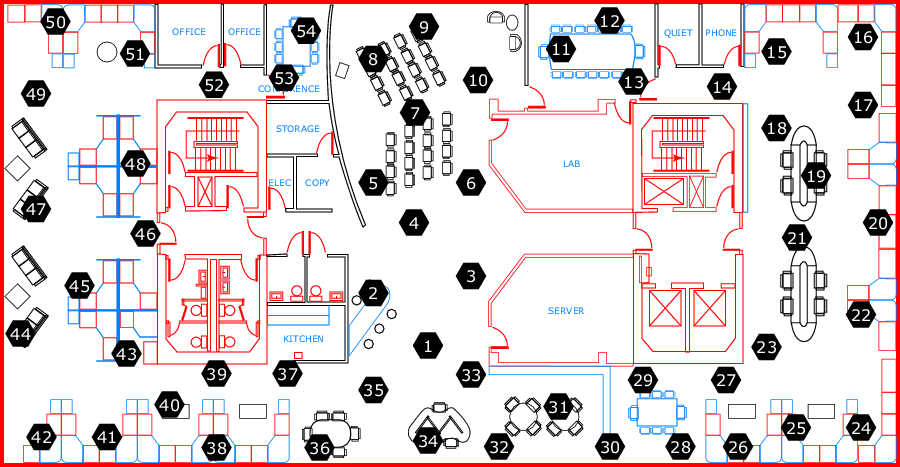
\includegraphics[width=0.13\textwidth,
                      height=0.08\textwidth]{figures/lab.png}};
  \node[inner sep=0pt,label=below:{\tiny Data locations},draw] (data) at (-4.25,-0.3)
    {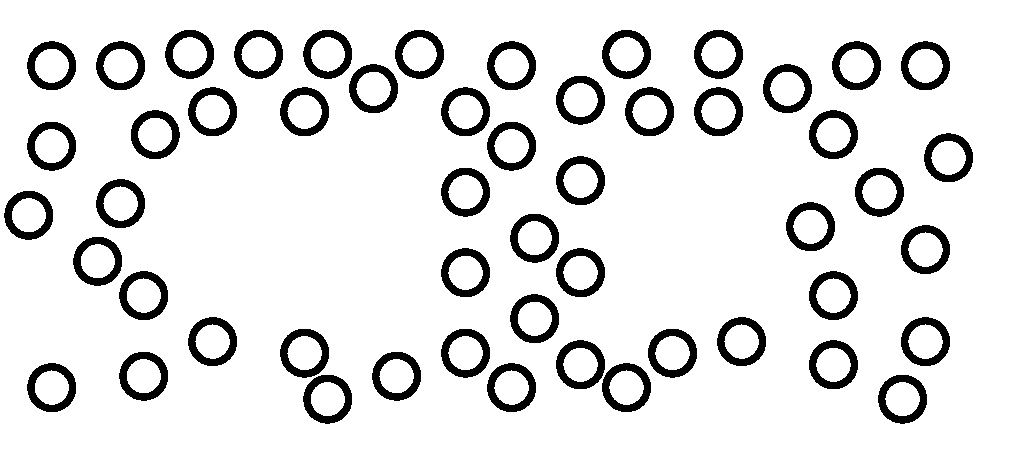
\includegraphics[width=0.13\textwidth,
                      height=0.08\textwidth]{figures/locations.pdf}};
  \node[inner sep=0pt,label=below:{\tiny Functional inference 
                                   (for $\estsysop$)},draw] (inference) at (-0.5,-0.3)
    {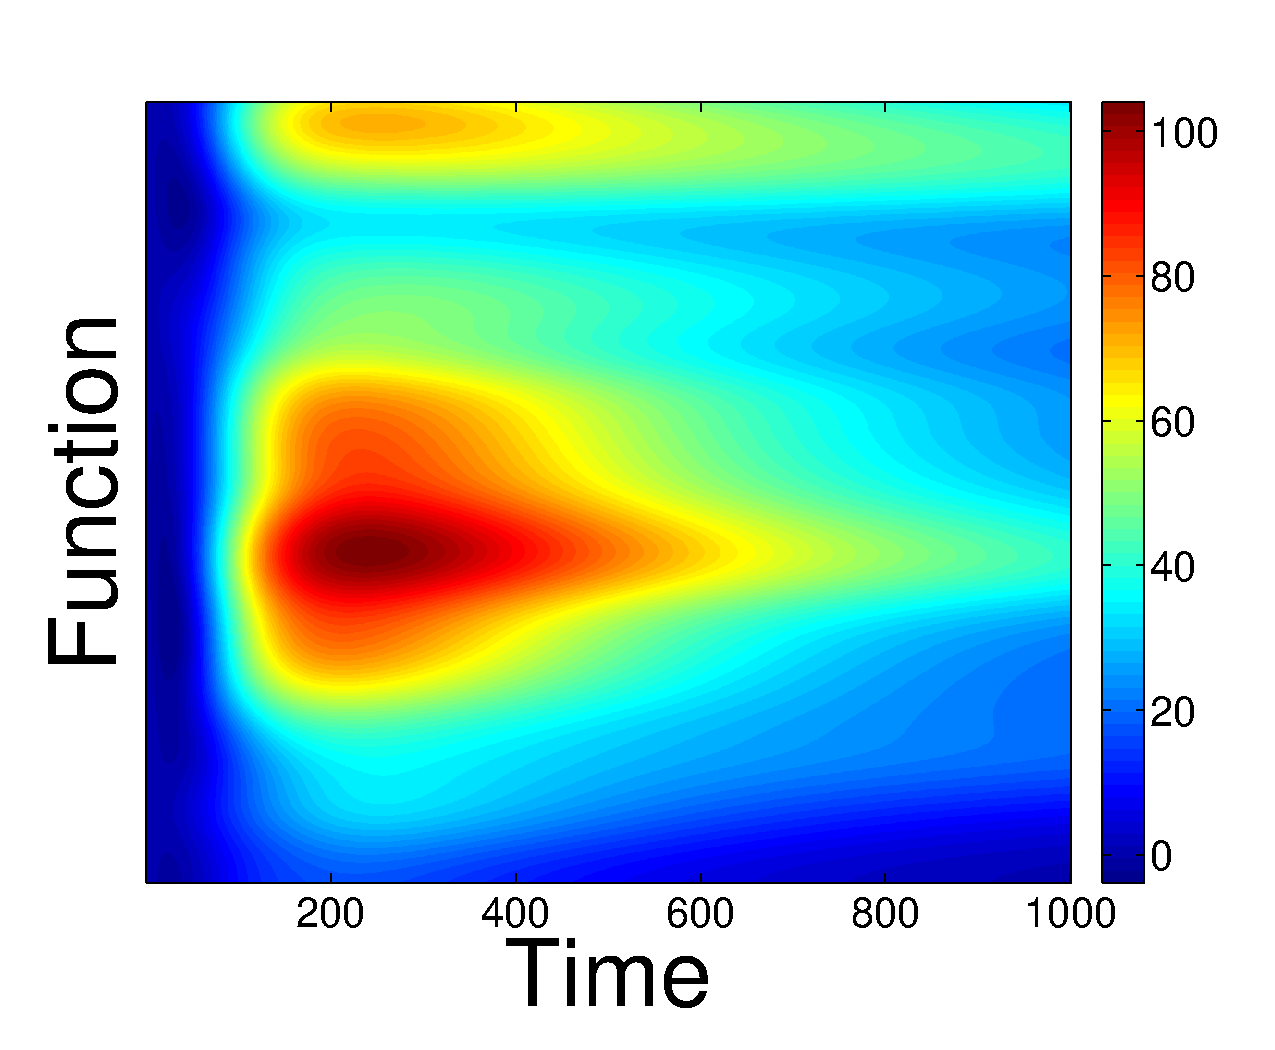
\includegraphics[trim=2.4cm 2.6cm 3.4cm 1.5cm,clip,
                      width=0.13\textwidth,
                      height=0.08\textwidth]{figures/kernel_evol_cauchy.pdf}};    
  \node[inner sep=0pt,label={[align=center]
       below:{\tiny Sensor location selection after\\[-1.7\jot]
              \tiny basis decomposition ($\minmeas=3$)}},draw] 
       (sensors) at (3.25,-0.3)
       {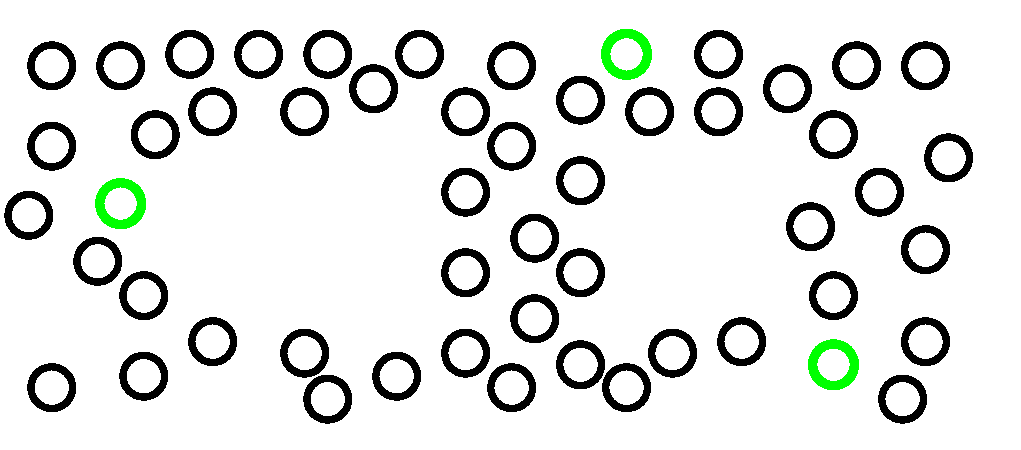
\includegraphics[width=0.13\textwidth,
                         height=0.08\textwidth]{figures/locations_sensors.pdf}};                          
  \node[inner sep=0pt,label=below:{\tiny Physical sensor placement},draw] (placement) at (6.75,-0.3)
    {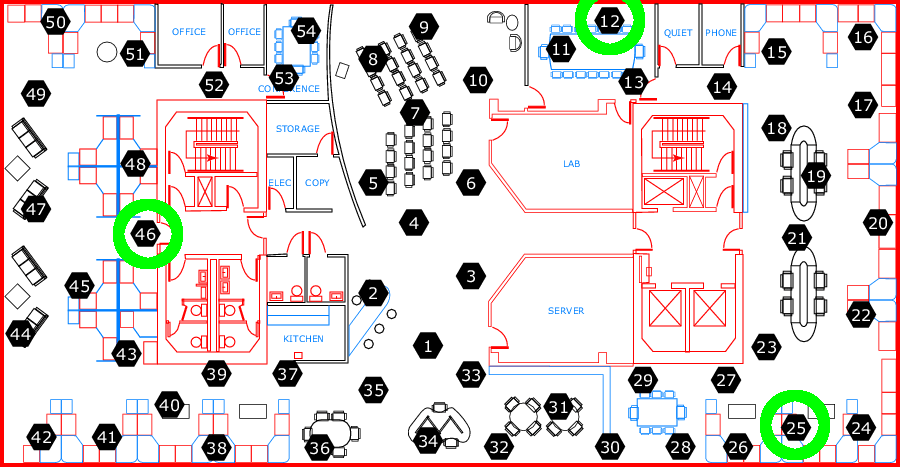
\includegraphics[width=0.13\textwidth,
                      height=0.08\textwidth]{figures/lab_sensors2.png}};                                                
  \path[every node/.style={font=\sffamily\small}]
    (physical) edge node [right] {} (data)
    (data) edge node [right] {} (inference)
    (inference) edge node [right] {} (sensors)
    (sensors) edge node [right] {} (placement);
\end{tikzpicture}

} % end framebox
} % end resizebox
\caption{
Overall description of how the kernel observer fits in the sensing framework. Physical 
locations are mapped to data locations, over which historical data is collected 
as a time series. Functional inference is performed over $\fspaceApprox$ to 
solve for $\estsysop$. The measurement operator $\empK$ is then computed 
(see Figure \ref{fig:sensplace}), leading to sensor placement. 
}\label{fig:overall_system}

\end{figure*}


\begin{figure*}[ht!]
  \begin{minipage}{\textwidth}
  \centering
  \begin{minipage}{0.47\textwidth}
  \resizebox{1\textwidth}{!}{
  \framebox[1.2\textwidth]{  
  \begin{tikzpicture}[scale=1.0, every node/.style={minimum size=1cm},on grid]    
	\begin{scope}[scale=\diagscale, xshift=-250, yshift=0]
		% The frame:
		\fill[white,fill opacity=.85] (0,0) rectangle (7,7); % Opacity
		\draw[black, thin] (0,0) rectangle (7,7); 
		 % Agents:
		\draw [fill=red]
			(4.7,2.7) circle (.2) % Firms
			(2,2) circle (.2) % Households
			(3.5,4.6) circle (.2); % Banks
		\fill[black]
			(0.5,6.5) node[right, scale=\diagtexttop] { \textbf{Compute cyclic index:}}
			(0.7,5.8) node[right, scale=\diagtexttop]
			{$\boldsymbol\minmeas = \mathbf{2}$}
			(4.5,2.1) node[right, scale=\diagtext]{$\boldsymbol\fmap(\mathbf{c_3})$}
			(2.5,1.4) node[left, scale=\diagtext]{$\boldsymbol\fmap(\mathbf{c_2})$}
			(3.5,4.6) node [above, scale=\diagtext] {$\boldsymbol\fmap(\mathbf{c_1})$}
			;
        % draw lines representing possible choices of decomposition                
        \draw[thick](1.3,4.1) to (6.5,4.1);
        \draw[thick](2.2,0.5) to (6.5,5.4);
        \draw[thick](2.5,0.5) to (2.5,5.3);
	\end{scope} 
	\begin{scope}[scale=\diagscale, xshift=0, yshift=0]
		% The frame:
		\draw[black, thin] (0,0) rectangle (7,7); 
		% Agents:
		\draw [fill=blue]
			(4.7,2.7) circle (.2) % Firms
			(2,2) circle (.2); % Households
		\draw [fill=green]			
			(3.5,4.6) circle (.2); % Banks
		 % Labels:
		\fill[black]
		        (0.5,6.5) node[right, scale=\diagtexttop] { \textbf{Compute meas. map:}}
			(0.7,5.8) node[right, scale=\diagtexttop]
			{$\boldsymbol\measmap =[\mathbf\linvec_1, 
			                        \mathbf\linvec_2]^T\boldsymbol\JorP^{-1}$}
% 			(4.5,2.1) node[right, scale=\diagtext]{$\boldsymbol\fmap(\mathbf{c_3})$}
% 			(2.5,1.4) node[left, scale=\diagtext]{$\boldsymbol\fmap(\mathbf{c_2})$}
% 			(3.5,4.6) node [above, scale=\diagtext] {$\boldsymbol\fmap(\mathbf{c_1})$}
			;
	\end{scope} 
	\begin{scope}[scale=\diagscale, xshift=250, yshift=0]
		% The frame:
		\draw[black, thin] (0,0) rectangle (7,7); 
		% Agents:
		\draw [fill=blue, opacity=0.4]
			(4.7,2.7) circle (.2) 
			(2,2) circle (.2)
			;
		\draw [fill=blue]
			(3.2,2) rectangle (3.55,2.35)
			; 
			\node (one) at (3.37,1.5) {\scriptsize$ 1 $};
		\draw [fill=green, opacity=0.4]
			(3.5,4.6) circle (.2)
			;
		\draw [fill=green]			
			(3.0,4.0) rectangle (3.35,4.35)
			;
			\node (two) at (3.17,3.5) {\scriptsize$ 2 $};
		\fill[black]
		        (0.5,6.5) node[right, scale=\diagtexttop] { \textbf{Sensor loc. selection:}}
			(0.7,5.8) node[right, scale=\diagtexttop]
			{$\mathbf{x_1, \ x_2\in}\boldsymbol\dom \boldsymbol\Rightarrow \empKShadFull$}
% 			(4.5,2.1) node[right, scale=\diagtext]{$\boldsymbol\fmap(\mathbf{c_3})$}
% 			(4.5,2.1) node[right, scale=\diagtext]{$\boldsymbol\fmap(\mathbf{x_2})$}
% 			(2.5,1.4) node[left, scale=\diagtext]{$\boldsymbol\fmap(\mathbf{c_2})$}
% 			(1.4,4.7) node[right, scale=\diagtext]{$\boldsymbol\fmap(\mathbf{x_1})$}
% 			(3.5,4.6) node [above, scale=\diagtext] {$\boldsymbol\fmap(\mathbf{c_1})$}
			;
	\end{scope}	
  \end{tikzpicture}
  } % end framebox
  } % end resizebox  
  \end{minipage}
  \begin{minipage}{0.47\textwidth}
  \resizebox{1\textwidth}{!}{
  \framebox[1.2\textwidth]{  
  \begin{tikzpicture}[scale=1.0, every node/.style={minimum size=1cm},on grid]  
	\begin{scope}[scale=\diagscale, xshift=-150, yshift=0]
		% The frame:
		\fill[white,fill opacity=.85] (0,0) rectangle (7,7); % Opacity
		\draw[black, thin] (0,0) rectangle (7,7); 
		 % Agents:
		\draw [fill=red]
			(4.7,2.7) circle (.2) % Firms
			(2,2) circle (.2) % Households
			(3.5,4.6) circle (.2); % Banks
		\fill[black]
			(0.5,6.5) node[right, scale=\diagtexttop]{\textbf{Compute cyclic index:}}
			(0.7,5.8) node[right, scale=\diagtexttop]
			{$\boldsymbol\minmeas = \mathbf{2}$}
			(4.5,2.1) node[right,scale=\diagtext]{$\boldsymbol\fmap(\mathbf{c_3})$}
			(2.5,1.4) node[left,scale=\diagtext]{$\boldsymbol\fmap(\mathbf{c_2})$}
			(3.5,4.6) node [above, scale=\diagtext] {$\boldsymbol\fmap(\mathbf{c_1})$};
        % draw lines representing possible choices of decomposition                
        \draw[thick](1.3,4.1) to (6.5,4.1);
        \draw[thick](2.2,0.5) to (6.5,5.4);
        \draw[thick](2.5,0.5) to (2.5,5.3);
	\end{scope} 
	\begin{scope}[scale=\diagscale, xshift=150, yshift=0]
		% The frame:
		\draw[black, thin] (0,0) rectangle (7,7); 
		% Agents:
		\draw [fill=blue, opacity=0.4]
			(4.7,2.7) circle (.2) % Firms
			(2,2) circle (.2)
			;
		\draw [fill=blue]
			(1.17,1.1) rectangle (1.17+0.35,1.1+0.35)
			(5.0,1.8) rectangle (5.35,2.15)
                        ;
           \node (one) at (1.31,0.7) {\scriptsize$ 1 $};
           \node (two) at (5.17,1.3) {\scriptsize$ 2 $};
		\draw [fill=green, opacity=0.4]
			(3.5,4.6) circle (.2)
			;
		\draw [fill=green]
                        (3.0,4.0) rectangle (3.35,4.35)
			;
			\node (three) at (3.17,3.5) {\scriptsize$ 3 $};
		 % Labels:
		\fill[black]
		        (0.5,6.5) node[right, scale=\diagtexttop] { \textbf{Random sampling:}}
			(0.7,5.8) node[right, scale=\diagtexttop]
			{$\mathbf{x_1, x_2, x_3\in} \boldsymbol\dom \Rightarrow \empKShadFull$}
% 			(4.5,2.1) node[right,scale=\diagtext]{$\boldsymbol\fmap(\mathbf{c_3})$}
% 			(2.5,1.4) node[left,scale=\diagtext]{$\boldsymbol\fmap(\mathbf{c_2})$}
% 			(3.5,4.6) node [above, scale=\diagtext] {$\boldsymbol\fmap(\mathbf{c_1})$}
			;
	\end{scope} 
  \end{tikzpicture}
  } % end framebox
  } % end resizebox                      
  %\captionof{figure}{Sensor selection using random sampling} \label{fig:sselec_rand}
  \end{minipage} 
  \end{minipage} 
  \caption{
  Diagram demonstrating sensor placement using the measurement map or random sampling approaches. 
  The circles represent data locations associated to bases (e.g. $c_j\Leftrightarrow\fmap(c_j)$) 
  and the squares represent sensor locations (e.g. $x_i\Leftrightarrow\fmap(x_i)$) .
  The cyclic index ($\minmeas=2$) indicates how many possible couplings of bases exist, 
  which can be represented 
  as a choice of $\binom{\ncent}{\minmeas}$ hyperplanes in $\dom$. If the measurement map is 
  computed (left), the correct couplings are chosen (green vs. blue), and a smaller number of sensors (2) can be placed.
  Alternatively, random sampling (right) is more computationally efficient, but generally
  requires more sensors (3). 
  }\label{fig:sensplace}
\end{figure*}



\subsection{Discussion of Theoretical Results}\label{sec:discussion}
The systems-theoretic approach taken in this paper reveals something rather surprising: functions with complex dynamics (with a small cyclic index) can be recovered with less sensor placements than functions with simpler dynamics. Although seemingly counterintuitive, it becomes clear that this is because complex dynamics, which are characterized by a lower geometric multiplicity of the eigenvalues, ensure that the orbit $\orbit := \{\dualopApprox\weight_{\tindex}\}_{\tindex\in\Tset}$ traverses a greater portion of $\R^{\ncent} \equiv \fspaceApprox$ and thus that fewer sensors can recover more geometric information. On the other hand, in `simpler' functional evolution, $\orbit$ evolves along strict subspaces of $\R^{\ncent}$, and so more independent sensors are required to infer the same amount of information. 

In the case described in Remark \ref{rem:1}, we have a set of centers $\shCent=\shCentLong$, which generate the bases $\Atoms = \{\fmap(c_1), \cdots , \fmap(c_{\ncent})\}$. Let the cyclic index be $\minmeas$: this implies that there exist $\minmeas$ subsets $\atomSubset{i}$ of $\Atoms$ with at least one element $\fmap(c_j)$ each, leading to $\binom{\ncent}{\minmeas}$ possible choices: Figure \ref{fig:sensplace} represents these choices as hyperplanes separating the subsets. 
The measurement map described in Alg. 1 in \cite{Kingravi16_NIPS} induces this \emph{decomposition of bases} $\Atoms = \{\atomSubset{1},\dots,\atomSubset{\minmeas}\}$ in polynomial time. Further, each subset $\atomSubset{i}$ is directly associated to a subset of centers $\centerSubset{i}\subset\shCent$, which allows us to pick targeted sensor locations $x_i\in\dom$. In particular, for radially symmetric kernels such as the Gaussian, the centroid of the convex hull of $\centerSubset{i}$ is sufficient for generating a sensor placement. The measurement map is a significant theoretical insight into sensor placement for dynamically changing environments, because it directly takes into account the dynamics of the process. Of course, in practice, this may be too expensive for approximate feature spaces with $\ncent$ very large, so one can use random sampling to generate the sensor locations instead, at the cost of $\nsamp$ being larger than $\minmeas$. The advantage here though is that since random sampling is computationally inexpensive, different choices of sensor placements can be generated and evaluated relatively quickly.

Another point to note is that since the collection of bases $\{\fmapApprox_i(x)\}_{i=1}^{\ncent}$ determines the richness of the function space $\fspaceApprox\approx\fspace$ we operate in, it determines the fidelity of the model approximation to the true time-varying function. As a consequence, observability of the system in $\fspaceApprox$ refers to the best possible approximation in $\fspaceApprox$. The greater the number of bases, the higher the dimensionality, which results in greater model fidelity, but which may require a much greater number of measurements for state recovery. This is where the lower bounds presented in the paper are particularly useful, because they show that for functional evolutions corresponding to certain $\dualopApprox$, \emph{the number of sensor placements are essentially independent of the dimensionality $\ncent$}, but depend rather on the cyclic index of $\dualopApprox$.

Figure \ref{fig:overall_system} gives an overall picture on the process of generating a kernel observer, while Figure \ref{fig:sensplace} gives two approaches to sensor selection in our framework. The measurement map approach can generate a smaller set of sensors than the random placement approach, but comes at an additional computational cost. 

\subsection{Random Sensor Placement}\label{sec:random_results}
We now elaborate on how the challenging problem of sensor placement can be tackled through random selection. This process of random selection is a product of the kernel observer model described above. We present the theoretical background required to prove Theorem \ref{thm:r1}, which states the expected number of randomly placed sensors required to monitor a given spatiotemporal process, and Theorem \ref{thm:r2}, which determines the probability with which optimal sensor placement is ensured given that, $\nsamp$ number of sensors have been placed. 
%Otherwise to the best of our knowledge there does not exist any sensor placement design based on random selection.%Thus, the kernel observer is a modeling solution for spatiotemporal processes that also guides deterministic as well as random placement of sensors.

As discussed earlier, we work with an approximate feature space $ \fspaceApprox $, with the corresponding transition operator $ \dualopApprox: \fspaceApprox \rightarrow \fspaceApprox $, representing finite-dimensional functional evolution. To achieve observability for the pair ($ \dualopApprox , \empK $), row vectors of the corresponding observability matrix, $ \Obs $, should form the basis for the $ \R^\ncent $-dimensional space $ \fspaceApprox $. According to the rational canonical structure Theorem \cite{wonham1974linear}, $\dualopApprox$ can successively decompose the dual space $ \R^\ncent $ into subspaces, $\linspace_i \subset \linspace$, $i\in \{1,\dots,\minmeas\}$, with properties, i) $\linspace = \linspace_1 \oplus ... \oplus \linspace_{\minmeas}$, ii) $\dualopApprox\linspace_i \subset \linspace_i$, and iii) $\dualopApprox|\linspace_i, i \in \{1,\dots,\minmeas\}$, are cyclic. The integer $\minmeas$ is unique and is called the \emph{cyclic index of $\dualopApprox$}.  Each of these properties contribute towards the theorem on the number of random samples required to achieve observability. The first property shows that the space $ \R^\ncent $ can be decomposed into $ \ell $ independent subspaces. The second property shows that the vector $ \linvec_i \in \linspace_i $ stays in $ \linspace_i $ even when operated upon by $ \dualopApprox $. Thus, to generate bases for $ \R^\ncent $, one needs at least $ \ell $ vectors, say, $ \linvec_1, \dots,\linvec_\ell $, with respect to each subspace $ \linspace_1,\dots,\linspace_\ell $. This holds due to the third property, but requires that the vectors  $ \linvec_1, \dots,\linvec_\ell, $ are the cyclic generators of their corresponding subspaces. Our analysis is based on whether a randomly selected sensor can generate a cyclic generator. To examine this, recall that a row vector $ \empK_{(i)} $ generated by a randomly selected sensor location $ x_i $ takes the form,
\begin{equation}\label{eq:rowvec}
\empK_{(i)} = \bbm k(x_i,c_1),\dots,k(x_i,c_\ncent) \ebm.
\end{equation}
Here, for radial kernels for example, the entries corresponding to the centers closer to $ x_i $ tend to be non-zero, whereas the others tend to be zero. 
% 	Note this holds since in general kernel function depends upon the metric of distance between its argument, for example the squared exponential kernel. 
% 	This limits the capability of a cyclic generator being obtained from a random sensor, however the latter certainly generates a non-zero entry for a closest sensor data point. 
The rows $\empK_{(i)}$ from random sensor placement must be able to generate a basis for a subspace $ \linspace_i $, and thus must be cyclic generators.  We will derive the expected number of random sensor placements sufficient for observability for the case where $ \dualopApprox = \JorLa $ and then attempt to generalize the result for any $ \dualopApprox $. Note $ \JorLa $ is a block diagonal Jordan form.  In this case, the cyclic generator for each subspace $ 
\linspace_i $, is a vector $ \linvec_i $ with non-zero entries corresponding to the leading entry of the Jordan blocks of $ 
\linspace_i $. 
%An example of a subspace, and  its cyclic generator is, 
%\begin{align}
%\linspace_1 & = \begin{bmatrix}{
%1 & 1 & 0 & 0\\
%0 & 1 & 1 & 0\\
%0 & 0 & 1 & 0\\
%0 & 0 & 0 & 2}
%\end{bmatrix}, \quad  \linvec_1 = \begin{bmatrix}{
%0 \\
%0 \\
%s \\
%s'},
%\end{bmatrix},  \nonumber 
%\end{align}
%where $s,s'$ are non-zero. 

Overall, our construction is as follows: for each subspace $ \linspace_i $, let $ \shCent_{\linspace_i} \subset \shCent $ be the centers corresponding to those leading entry of Jordan blocks: then the minimum number of random samples required to generate the bases for $ \linspace_i $ is equal to the number of Jordan blocks comprising $ \linspace_i $. Altogether, the minimum number of random samples required to generate a basis for $ \R^\ncent $ is equal to the total number of Jordan blocks in $ \dualopApprox $. Let $ \rands $ be the total number of Jordan blocks in $ \dualopApprox  $, then
%	For entire space we obtain the measurement map $ \measmap = [\linvec_1^T, \linvec_2^T,...,\linvec_{\minmeas}^T]^T $.
\begin{equation}\label{rands}
\rands = \sum_{\lambda \in \sigma(\dualopApprox)} \gamma_{\dualopApprox}(\lambda) \qquad %\geomMult_\lambda
\end{equation}
where $\sigma(\dualopApprox) $ represents the spectrum of $ \dualopApprox $, whose elements are the eigenvalues of $ \dualopApprox $, and $ \gamma_{\dualopApprox}(\lambda) $ is the geometric multiplicity corresponding to the eigenvalue $ \lambda $, which is also equal to the total number of Jordan blocks corresponding to the eigenvalue $ \lambda $. Define a set of centers $ \shCent_\rands $ with elements $ \{c_1, c_2,\dots, c_\rands\} $, to be the centers corresponding to the leading entries of  the Jordan blocks.
For sensor location $x\in\dom$, and $ \epsilon > 0 $, let $\kernel(x, c_j) > \epsilon$, denote the region $\dom_j\subset\dom$, such that the kernel evaluation with respect to center $c_j$ is greater than $\e$, that is $ \dom_j \equiv \{x\in \dom:\kernel(x, c_j) > \epsilon\} $. We define
$ p_{\e} $ as
\begin{equation}\label{ppp}
p_{\e} = \min_{c_j \in \shCent_\rands} \frac{\measure(\kernel(x, c_j) > \epsilon)}{\measure(\dom)},
\end{equation}
where $\measure$ is a measure in the real analysis sense. Hence, $p_{\e}$ corresponds to a lower bound on the probability that a random sample lies within the $ \epsilon-$shaded region of a particular center $ c_j$. With all of this in place, we can prove the following theorem. 
\begin{theorem}\label{thm:r1}
	Given the spatiotemporal function $ f(x,\tindex) $ with $ x \in \dom \subseteq  \mathbb{R}^\dimI, \tindex\in \mathbb{Z}^+  $ its kernel observer model \eqref{k_measure}, and a tolerance parameter $\e>0$, the expected number of randomly placed sensor locations required to achieve observability for the pair $ (\empK,\dualopApprox) $ is $ \rands/{p_{\e}} $ where $ \rands $ is the summation over geometric multiplicities of each $ \lambda \in \sigma(\dualopApprox) $  given by  (\ref{rands}).
\end{theorem}
\begin{theorem}\label{thm:r2}
	Given the spatiotemporal function $ f(x,\tindex) $ with $ x \in \dom \subseteq  \mathbb{R}^\dimI, \tindex\in \mathbb{Z}^+  $, its kernel observer model \eqref{k_measure}, a tolerance parameter $\e>0$, summation over geometric multiplicities of each $ \lambda \in \sigma(\dualopApprox) $ denoted by $ \rands  $ as in  (\ref{rands}), and a constant $ \delta \in (0,1] $, the probability that pair $ (\empK, \dualopApprox) $ is unobservable after the selection of $ \nsamp $ random sensors is at most $ e^{\frac{-1}{2}(\nsamp p_{\e}-2\rands)} $, where $ p_{\e} $ is given by (\ref{ppp}) and \rr{$ \nsamp > 2\rands/p_{\e} $}.
\end{theorem}
For the case when $ \dualopApprox \neq \JorLa $, a change of basis can be used to obtain $ \JorLa = P^{-1}\dualopApprox P $, where $ P $ is the projection map. There are two challenges in performing the above analysis for $\JorLa$ so obtained: first, the leading entries of Jordan blocks do not directly correspond to the centers $\{ c_1,\dots,c_\ncent\}$ which was the case for $ \dualopApprox = \JorLa $. Second, although we can obtain the transformation of the row vector (\ref{eq:rowvec}) using the projection map $P$, we can no longer arrive at the definition of the probability $p_{\e}$ as in  (\ref{ppp}). The existence of the similarity transform hints that the results in Theorems \ref{thm:r1}-\ref{thm:r2} should hold for any $ \dualopApprox$, but the mathematical tools utilized in the paper seem to be insufficient to prove them. However, we present some empirical evidence for these claims for when $ \dualopApprox \neq \JorLa $  in the empirical results section.%Section \cite{Maske18_ACC}.


\subsection{Generalizing Across Similar Spatiotemporally Evolving Systems} \label{sec:egp}
Building on the Kernel Observers method, let us introduce Evolving Gaussian Processes (E-GP). The primary novelty in this method of generating a model is learning an $\dualopApprox$ matrix for \emph{multiple} systems. The ultimate goal of this research would be to generate highly efficient machine learning models that can be used instead of the costly numerical simulations for design and autonomy purposes. This would be a major success for the design and control of complex physical systems, such as soft robotics, as they would significantly reduce the cost and resources required in simulations. The ability to generalize across different physical situations, is critical. This is a difficult problem, as it requires that the model have the capability to actually learn the underlying physics and not just input-output relationships. For example, in the context of fluid flows, these models must be able to predict fluid dynamics at different conditions (e.g. Reynolds number) than the training data. E-GP, as far as the authors know, was the first machine learning method to generalize across spatiotemporally evolving systems of such complexity using end-to-end data.

We found that the class of functional evolutions $\mathbb{F}$ defined by linear Markovian transitions in a RKHS is still sufficient to model the nonlinear Navier Stokes equations which govern fluid dynamics, since the unknown map $\fmap$ allows us to model highly nonlinear dynamics in the input space. However, we do expect that phenomena such as bifurcation or turbulence will require nonlinear mappings $\fspace$. There are three steps to generate an E-GP model:

\begin{enumerate}
	\item After picking the kernel and estimating the bandwidth hyperparameter $\s$ (we utilize the maximum likelihood approach, although other approaches can be used), find an optimal basis vector set $\shCent$ using the algorithm in \cite{csato2002sparse}.
	\item Use Gaussian process inference to find weight vectors for each time-step in the training set(s), generating the sequence $\weight_\tindex, \tindex=1,\dots,T$ for each system. A uniform time-step makes next step easier but can be worked around for non-uniform data sets
	\item Using the weight trajectory, use matrix least-squares with the equation $\dualopApprox [\weight_1,\weight_2, ...,\weight_{T-1}] = [\weight_2,\weight_3,...,\weight_T]$ to solve for $\dualopApprox$.
	\item To generate a multi-system model, concatenate the weight trajectories from each similar system in the least-squares computation of $\dualopApprox$. That is, let $W_{\theta} = [\weight_1^{(\theta)},\weight_2^{(\theta)}, ...,\weight_{n-1}^{(\theta)}]$ and $W_{\theta}' = [\weight_2^{(\theta)},\weight_3^{(\theta)}, ...,\weight_n^{(\theta)}]$ be the weight trajectory and next weight trajectory for some parameter . Then we solve the least-squares problem $\dualopApprox = [W_{\theta_1},\dots,W_{\theta_n}] = [W_{\theta}',\dots,W_{\theta_n}']$
\end{enumerate}

For the sake of defining when it is appropriate to expect this method to be able to generalize across different spatiotemporally evolving systems, we shall define what it means for two fluid flows to be \emph{similar}. In configuring a fluid dynamics simulation, a set of quantifiable parameters are defined. Two dynamical fluid systems $S_1$ and $S_2$ are considered \emph{similar} if they have  the same configuration of parameters and differ only in the value of at most one parameter. Furthermore, we require that the parameter be continuously variable, and that any observable quantity in the domain of the system vary smoothly as that parameter varies from its value in $S_1$ to its value in $S_2$. For example, for fluids flowing past identical cylinders, the Reynolds number associated with the free stream velocity may be varied to produce similar systems. However, to replace the system's cylinder with a triangle would be to qualitatively change the configuration of the system parameters, and thus would produce a non-similar system.

Unlike neural networks, the weights in an E-GP do not exist in some abstract, difficult-to-comprehend space, but are associated with kernel centers in specific locations in the domain. We refer to this attribute of E-GPs as the \emph{spatial encoding} property. This property is an extremely valuable tool for gaining insight into the learned model works:
\begin{enumerate}
	\item By plotting which kernel centers are associated with which invariant subspaces in the transition matrix, one can visualize where the eigenfunctions are found and how the dynamic modes are separated spatially
	\item By plotting arrows from center $c_j$ to $c_i$ for each of the largest elements $\hat a_{ij}$ of $\dualopApprox$, one can visualize how different areas of the domain influence each other's evolution.
	\item By performing an eigendecomposition of the $\dualopApprox$ matrix, and transforming the eigenvectors back from the weight space to the function space, one can obtain the Koopman modes (and associated eigenvalues) of the system (see next section)
\end{enumerate}


\subsection{\rr{Spectral Analysis of Evolving Gaussian Process Model and Resulting Algorithms}}

\rr{For a general dynamical system $f_{\tindex+1} = \mathbb{F}(f_{\tindex})$ defined on a state space (for us, an RKHS, i.e. $f\in\fspace$), we can define an arbitrary, vector-valued \emph{observable} $g : \fspace \to \R^{\nsamp}$. Note that the space of observables $g$ is a vector space. The Koopman operator $U$ is defined to be the operator on the space of observables such that}
\begin{align} \eqlabel{koopman_operator}
U g(f_{\tindex}) = g(\mathbb{F}(f_{\tindex})) = g(f_{\tindex+1})
\end{align}
\rr{This operator is clearly linear from its definition, and thus it is reasonable to examine its spectral properties. The special observables $\phi : \fspace \to \C$ that have the property}
\begin{align} \eqlabel{koopman_eigenfunctions}
U \phi(f_{\tindex}) = \phi(\mathbb{F}(f_{\tindex})) = \phi(f_{\tindex+1}) = \lambda \phi(f_{\tindex})
\end{align}
\rr{are the eigenfunctions of $U$, and the associated $\lambda$ are the eigenvalues. Suppose now we have a vector-valued observable $u(\fspaceEl,x)$, where $x\in\dom$ and $\fspaceEl\in\fspace$.}

\begin{definition}
	\rr{The Koopman mode $s(x)$ at isolated eigenvalue $\lambda$ of algebraic multiplicity 1 is the projection of $u(f,x)$ onto the eigenfunction $\phi_{\lambda}(\fspaceEl)$ of $U$ at $\lambda$. \cite{mezic2013analysis}}
\end{definition}

\rr{As previously shown by Rowley in 2009 \cite{rowley2009spectral}, the modes produced by the Dynamic Mode Decomposition (DMD) algorithm constitute a subset of Koopman modes. Mezic (2013) showed that there exists, in principle if not in practice, a rigorous method for computing the full set of Koopman modes by a method known as generalized Laplace analysis (GLA). We have generated a number of results interpreting the E-GP model in terms of Koopman operator theory, culminating in the proof that the eigenvalues and eigenvectors of $\dualopApprox$ are related to the Koopman eigenvalues and modes.}

\begin{proposition}\label{thm:ApproxObsv}
	\rr{Let $\fspace$ be a RKHS with  an approximate feature space $\fspaceApprox$, and let $u(\fspaceEl,x)$ be an observable in the Koopman sense with respect to the dynamical system $f_{\tindex+1} = \mathbb{F}(f_{\tindex})$ in $\fspace$. Then $\hat u(\fspaceEl,x) \coloneqq u(\fspaceApproxEl,x)$, where $\fspaceApproxEl$ is the projection of $\fspaceEl\in\fspace$ onto $\fspaceApprox$, is also an observable.}
	%Given a RKHS $\fspace$ and an approximate feature space $\fspaceApprox$ which has finite dimension $\ncent$, the projection $\fmapApprox : \fspace \to \R^\ncent$ from the RKHS to the dual space of $\fspaceApprox$ is an observable in the Koopman sense with respect to the dynamical system $f_{\tindex+1} = \mathbb{F}(f_{\tindex})$
\end{proposition}

This follows from the fact that the projection from the function space to its subspace is well-defined when the $\fmapApprox_i$ are independent. Now, Koopman modes of observables are of interest because they are akin to the eigenvector expansions utilized in linear dynamics. If we separate the Koopman operator into $U = U_s + U_r$ where $U_s$ has a pure point spectrum and $U_r$ has a pure continuous spectrum, then we can write
\begin{align} \eqlabel{spectral_expansion}
U^t u(\fspaceEl,x) = \mathbf{u^{\ast}}(\fspaceEl,x) + \sum_{j=1}^k \lambda_j^t \phi_j(\fspaceEl) s_j (x)  +  U_r^t u(\fspaceEl,x)
\end{align}
where $\mathbf{u^{\ast}}(x)$ represents the time-averaged of part of the field, which corresponds with $\lambda=1$ (see GLA in \cite{mezic2013analysis}). The continuous-spectrum component is usually discarded/neglected since it represents the part of the field that is genuinely aperiodic (or chaotic) in time, which could be modeled as a stochastic process \cite{mezic2013analysis}. Now, from this expansion we can prove that:
\begin{proposition}\label{thm:ApproxModes}
	Let $u(\fspaceEl,x)$ and $\hat u(\fspaceEl,x)$ be observables as in Proposition \ref{thm:ApproxObsv}, and $s_j(x)$ be the Koopman modes associated with the projection of the former onto the eigenfunctions $\phi_j$ of $U$ at $\lambda_j$. Then the Koopman modes associated with $\hat u$ are
	\begin{align}
	\hat s_j(x) = \frac{\phi_j(\fspaceApproxEl)}{\phi_j(\fspaceEl)} s_j(x)
	\end{align}
\end{proposition}
\begin{proof}
	Using the spectral expansion and the definition of the observables, we have
$$U^t \hat u(\fspaceEl,x) = U^t u(\fspaceApproxEl,x) = \mathbf{u^{\ast}}(\fspaceApproxEl,x) + \sum_{j=1}^k \lambda_j^t \phi_j(\fspaceApproxEl) s_j (x)  +  U_r^t u(\fspaceApproxEl,x)$$
$$ = \hat u^{\ast}(\fspaceEl,x) + \sum_{j=1}^k \lambda_j^t \phi_j(\fspaceEl) \hat s_j (x)  +  U_r^t \hat u(\fspaceEl,x) $$
It is easy to see that this must be the spectral expansion of $\hat u(\fspaceEl,x)$
\end{proof}

Note that this means the modes of the two observables are identical in shape (only differing by a multiplicative constant). In the exceptional case that $\phi_j(\fspaceEl)=0$, the GLA method is unable to compute $s_j (x)$ anyway, so that is not an issue for this proposition. The final step in our analysis is to connect the Koopman modes with the spectral decomposition of  our model's $\dualopApprox$ operator in the dual space.

\begin{theorem}\label{thm:DualApproxModes}
	In an E-GP or KO model of the dynamical system $ f_{\tindex+1} = \sysop f_{\tindex}$, the eigenvalues of $\dualopApprox$ are a subset of the eigenvalues of the Koopman operator. Furthermore, if the observable $u(\fspaceEl,x)$ is the evaluation operator, $u(\fspaceEl,x) = \fspaceEl(x)$, then the eigenvectors $v_j$ of $\dualopApprox$ are related to the Koopman modes of the observable by
	$$s_j (x) = \frac{\phi_j(\fspaceEl)}{\phi_j(\fspaceApproxEl)} \obsMatRow(x) \cdot v_j$$
\end{theorem}
\begin{proof}
	It should be clear that, as long as the projection onto the approximate feature space is well defined, that $\weight(f_{\tindex}) \coloneqq \weight_{\tindex} $ is an observable. Then if we let $\phi_j(\fspaceEl) = \langle \weight(\fspaceEl), q_j \rangle$, where $q_j$ are eigenvectors of the adjoint $\dualopApprox^{\ast}$ (that is, $\dualopApprox^{\ast} q_j = \bar \lambda_j q_j$), then $\phi_j$ is an eigenfunction of the Koopman operator: $U \phi_j(f_{\tindex}) = \langle \weight(f_{\tindex+1}), q_j \rangle = \langle \weight_{\tindex+1}, q_j \rangle = \langle \dualopApprox \weight_{\tindex}, q_j \rangle =  \langle \weight_{\tindex}, \dualopApprox^{\ast} q_j \rangle =  \lambda_j \langle \weight_{\tindex}, q_j \rangle =  \lambda_j \phi_j(f_{\tindex})$. This shows that the eigenvalues of $\dualopApprox$ correspond with that of the Koopman operator.
	
	In the case that $u(\fspaceEl,x) = \fspaceEl(x)$, we have the relationship $\hat u(\fspaceEl,x) = \fspaceApproxEl(x) = \obsMatRow(x) \cdot \weight(\fspaceEl)$.
\end{proof}

In the end, we have established a direct connection between the spectral decomposition of the transition matrix in the dual space of the approximate feature space and the Koopman modes, eigenfunctions, and eigenvalues. 

\begin{corollary}
	Suppose, given an $\e>0$, we are able to find an approximate feature space $\fspaceApprox$ such that for all $\fspaceEl\in\fspace$ there exists $\fspaceApproxEl\in\fspaceApprox$ such that $\|\fspaceEl - \fspaceApproxEl\| < \e$. Then, if $\phi_j(\fspaceEl) \neq 0$, there exists an approximate feature space such that $\obsMatRow(x) \cdot v_j$ (where $v_j$ is an eigenvector of the dual space transition matrix $\dualopApprox$) is arbitrarily close to the Koopman mode $s_j(x)$
\end{corollary}
\begin{proof}
	Since $\phi_j$ is continuous, we can make $|\phi_j(\fspaceEl) - \phi_j(\fspaceApproxEl)|$ arbitrarily small, which means if $\phi_j{\fspaceEl} \neq 0$ we can make $\frac{\phi_j(\fspaceEl)}{\phi_j(\fspaceApproxEl)}$ arbitrarily close to 1. From Theorem \ref{thm:DualApproxModes} and the fact that $s_j\in\fspace$ means $s_j$ is bounded, we can conclude that $\obsMatRow(x) \cdot v_j$ can be made arbitrarily close to $s_j(x)$ everywhere in $\dom$. %choose $\delta$ such that $\|\fspaceEl - \fspaceApproxEl\| < \delta$ implies $|\phi_j(\fspaceEl) - \phi_j(\fspaceApproxEl)| < 
\end{proof}


%in an rkhs, f and fhat being close means they are pointwise close.

%It is well known that in the case in which the dynamical system is linear, such as $\weight_{\tindex+1} = \dualopApprox\weight_{\tindex}$, its matrix eigenvalues are eigenvalues of the associated Koopman operator. The associated Koopman eigenfunctions

%We can show that there exists a relationship between the 


\subsubsection{Invariant Subspaces}

\rr{One way of viewing the invariant subspaces concept (as described earlier) is say that information contained in an invariant subspace never leaves that invariant subspace. We hypothesize that the kernel centers associated with the invariant subspaces of a spatiotemporally evolving system are generally associated with spatial regions in the domain (and not just homogeneously spread all over and or mixed with the other invariant subspaces). This hypothesis makes sense both physically and mathematically. In physics, the \emph{principle of locality} states that an object is only directly influenced by its immediate surroundings \cite{berkovitz2007action}. If this is the case (and there is no reason to believe that it is not, apart from certain quantum dynamics situations), and the E-GP model accurately captures the physics of the system, then information (measurable phenomena) may only travel continuously from one point in the domain to another. Mathematically, since a value at any one point in the domain is influenced by the weights of multiple nearby centers, we would expect nearby centers to be connected dynamically, unless separated by ``plains'' where the values are indistinguishable from noise.}

\rr{When a square matrix is perfectly formed, the Jordan form of a $n\times n$ matrix $\dualopApprox$ is block diagonal, and therefore gives a decomposition of the $n$ dimensional Euclidean space into invariant subspaces of $\dualopApprox$. The cyclic index, which can be found by counting the geometric multiplicities of eigenvalues in $\dualopApprox$, gives the number of invariant subspaces. In reality, data-driven approximations of $\dualopApprox$ rarely give such easily interpretable properties. Hence, the need for an algorithm can divide the system into invariant subspaces even when the boundaries between them are ``fuzzy''.}

\rr{Each block in the Jordan normal form has a set of corresponding eigenvectors and an eigenvalue with geometric multiplicity. When we transform the former back into the domain space, we obtain complex-valued functions which are the Koopman modes of the system. These provide an image of what kind of structures we see in the dynamics. The eigenvalues describe the frequency with which these structures oscillate between their real and imaginary forms, as well as the exponential growth or decay of their magnitudes.} %In this section, we demonstrate our method on systems with eigenvalues primarily on the unit circle (neither growing nor decaying).


\subsubsection{$k$-Invariant Subspaces Clustering}
\rr{The intuition behind our $k$-invariant subspaces clustering algorithm is to replace the Euclidean distance in the $k$-means algorithm with a different metric of ``nearness'', namely one corresponding with the dynamic connections in the space. The $\dualopApprox$ matrix provides easy access to these: its rows $\dualopApprox_{i\ast}$ indicate which centers inform the i\textsuperscript{th} value of $\weight_{tindex+1}$, and its columns $\dualopApprox_{\ast j}$ indicate what centers will be informed by the j\textsuperscript{th} value of $\weight_{\tindex}$. However, these values do tend to be biased towards the eigenmodes with higher frequencies (i.e. those whose eigenvalues have a greater polar angle) and those which grow exponentially. To  control for this, we chose modify the eigenvalues of the matrix in the following way: (1) We zeroed any eigenvalue that is clearly inside (not on) the unit circle, (2) We unitized the remaining eigenvalues, and (3) We adjusted the frequency of the remaining eigenvalues on the unit circle to either $\pm \frac{\pi}{4}$. If the eigen-decomposition of the original was $\dualopApprox = UDU^{-1}$, then we can reconstruct a new matrix with our modified eigenvalues $\bar D$ as $\bar A = U\bar D U^{-1}$.}

\rr{Much like the pairwise-squared deviations of points formulation of the $k$-means clustering problem, we can now write our problem as}
$$\arg\max_S \sum_{i=1}^k \frac{1}{2|S_i|} \sum_{\substack{x_i \neq x_j \\ x_j,x_i\in S_i}} \bar A_{ij}^2 $$

This problem can be solved with the following algorithm:
\begin{figure}[t!]
	\begin{algorithm}[H]
		\caption{$k$-Invariant Subspaces Algorithm}
		\label{kinvsub}
		\begin{algorithmic}
				\WHILE{clusters have changed}   
				\FOR{each center $i$}
				\STATE {Find cluster $k$ which maximizes the score} $ \frac{1}{|S_k|} \left( \|\bar A_{i, S_k\setminus \{i\} } \|^2 + \|\bar A_{S_k\setminus \{i\},i} \|^2 \right)$
				\STATE Reassign center $i$ to cluster with highest score
				\ENDFOR
				\ENDWHILE   
				\STATE \textbf{return} clusters
		\end{algorithmic}
	\end{algorithm}
	\vspace{-0.2in}
\end{figure}



%\begin{figure}[t!]
%\begin{algorithm}
%
%	\begin{algorithmic}
%	%	\WHILE{clusters have changed}
%%		\FOR{each center $i$}
%%		%\STATE {find cluster $k$ which maximizes the score} $ \frac{1}{|S_k|} \left( \|\bar A_{i, S_k\setminus \{i\} } \|^2 + \|\bar A_{S_k\setminus \{i\},i} \|^2 \right)$
%%		\STATE reassign center $i$ to cluster with highest score
%%		\ENDFOR
%%		\ENDWHILE
%%		\STATE \textbf{return} clusters
%	\end{algorithmic}
%\end{algorithm}
%\end{figure}


\rr{Note the differences between this and the $k$-means clustering algorithm: first, we are \emph{maximizing} since the terms represent influence rather than distance. Secondly, in the possible case that $|S_k|=0$, we make the total value zero in order to avoid division by zero. Thirdly, we exclude centers' influence on themselves from the score by taking $S_k\setminus\{i\}$.}

\rr{This algorithm can be repeated as many times as desired with different random initial conditions, and the result which produces the highest score retained.}

\subsubsection{Scoring Paths for a Moving Agent}

\rr{Consider the problem of predicting the current state of a spatiotemporally-evolving function with a set of robots, each one of whom can only observe the phenomena partially. When there are sufficient such robots to cover the entire domain, there are many approaches in the coverage literature available for solving this problem \cite{hussein2006effective,hussein2007effective}. In those approaches, the robots figure out the best trajectories to create a network of connected sensors that can simultaneously observe the whole environment. However, when the number of robots is limited, full coverage of the domain is not possible. How a few robots whose combined sensors can only observe a small part of the domain can predict the state of the spatiotemporally-evolving function remains an open problem.  Here we consider a limiting case of this problem where only a single robot is available to observe the whole environment, but the robot has available to it an approximate model of the function learned through past experience Evolving Gaussian Processes.}

\rr{We will be using a Kalman filter in the weight space of the E-GP as described in previous sections. In order to determine where a moving agent should go in order to gather the measurements which will help it converge to the true state of the system quickest, we use information from the spectral analysis of the E-GP model. We postulate that the value of taking a measurement at a point in the domain with respect to a particular eigenvector is proportional to the following factors:}

\begin{enumerate}
	\item The spatial extent of the eigenvector. This can be taken to be equivalent to the area under the curve of the magnitude of the complex function corresponding to that eigenvector (normalized by the function peak)
	$$ SE_i = \frac{1}{\sup_x |v_i \hat\Phi(x)|} \int_X |v_i \hat\Phi(x)| dx $$
	This Riemman integral can of course be approximated by discretely partitioning the space. From this point of view, we can see that this expression represents what proportion of the domain is subject to variance due to the oscillation of this mode.
	
	\item The expected size of the measurement itself, which we take to be proportional to to $|v_i \hat \Phi(x)|$. This is included because greater measurements mean relatively greater correction to the state estimate.
	
	\item The ratio of the frequency with which that Koopman mode is visited to the frequency of its eigenvalue. This factor is included due to the aliasing effect, and is related to the concept of the Nyquist frequency. Modes with higher frequencies need to be visited more often than modes with lower frequencies.
	
	\item A discount factor equal to a decaying exponential of the number of times that eigenmode has been visited. This factor is included due to the exponential convergence of a Kernel Observer. The information gained by taking a measurement within the active area of a particular dynamic mode decreases exponentially the more measurements are taken.
\end{enumerate}

\rr{This scoring method allows one to decide the likeliest candidate amongst a large family of paths.}


\subsubsection{Generating High-Scoring Random Paths}

\rr{We propose the following algorithm for generating high-scoring paths:}
\begin{enumerate}
	\item Cluster the centers into invariant subspaces according to the $k$-invariant subspaces algorithm, with the best reasonable guess(es) for $k$. This is necessary in order that the robot may be sure it is keeping track of each of the independent subsystems.
	\item Within each cluster, select a waypoints at local maxima of the sum of the Koopman modes. These are where the best measurements may be taken.
	\item Generate a path by selecting waypoints randomly according to a weighting scheme. The weights are equal to the spatial extent of the clusters, multiplied by an exponential decay factor for the number of times each has been visited (see item 4 in the previous section)
\end{enumerate}
 